\documentclass[11pt]{article}

\usepackage[utf8]{inputenc}
\usepackage[T1]{fontenc}
%\usepackage[francais]{babel}
\usepackage[french]{babel}
\usepackage{eurosym}
\usepackage{lmodern}
\usepackage{boxedminipage}
\usepackage{moreverb}
\usepackage{microtype}
\usepackage{listings}
\lstset{
basicstyle=\small\ttfamily,
columns=flexible,
breaklines=true
}

\usepackage[pdftex]{graphicx}
\graphicspath{{./fig/}}
\usepackage[colorlinks,linkcolor=blue,citecolor=blue,pagebackref]{hyperref}
\usepackage{amsmath,amssymb,amsfonts,mathrsfs}
\usepackage[usenames,dvipsnames]{color}
\usepackage{float}
\usepackage{graphicx}
\usepackage{multirow}
\usepackage{pgfgantt}
\usepackage{multicol}
\usepackage{wrapfig,lipsum,booktabs}
\usepackage{tikz}
\usetikzlibrary{calc, arrows, shapes, fit}
\usetikzlibrary{positioning,intersections}
\usepackage{pgfplots}
\pgfplotsset{compat=1.8}

%for timing diagrams
% tikz for chronogram
\usepackage{tikz-timing}

%-----------------------------------------------------------------------
\usepackage[
text={15cm,21cm},
centering,
% showframe,
]{geometry}

\numberwithin{equation}{section}
\numberwithin{figure}{section}
%\renewcommand{\theequation}{\thesection.\arabic{equation}}
%\renewcommand{\thetable}{\thesection.\arabic{table}}

%-----------------------------------------------------------------------
% The following macros determine the part of the text that will actually
% be compiled. When the paper is completed, set all the macros to 0.

\def\withtoc{0}
   % "with table of contents (TOC)"
   % 0: without TOC
   % 1: with TOC

%-----------------------------------------------------------------------

\newcommand{\CAD}{c.-\`a-d.}
\newcommand{\PEX}{p.\,ex.}
\newcommand{\tocvspace}{-2.0ex}
\usepackage{xspace}
\newcommand{\syfala}{{Syfala}\xspace}
\newcommand{\todo}[1]{\footnote{#1}}

%-----------------------------------------------------------------------


\newcommand{\tcb}{\textcolor{blue}}
\newcommand{\tcg}{\textcolor{OliveGreen}}
\newcommand{\red}{\textcolor{red}}

\newcommand{\knownbug}[1]{ #1}

\newcommand{\adtname}{SytaRiot}

%-----------------------------------------------------------------------
\title{\Large\bf Developper documentation for  the Syfala project: \\ From Faust to FPGA}
\author{The Syfala Team}
\date{\today}
\begin{document}
\maketitle

\tableofcontents

\setcounter{section}{-1}
\newpage
\section{Very Quick Start}
Last update of this document: \today

\paragraph{Most recent version:} Syfala v7, Vivado 2020.2 and Faust $\geq$ 2.39.3\\

\begin{boxedminipage}{\textwidth}
  \begin{verbatim}
#make sure that vivado (v=2020.2) and Faust (v>2.39.3) are installed
#on your computer (see Syfala install documentation)
git clone https://github.com/inria-emeraude/syfala.git  my-clone-syfala
cd my-clone-syfala/
./syfala.tcl install
# connect the Zybo by USB with all switchs down (i.e. opposite to 
# ethernet connector plug) on LD0 side and blue jumper on JTAG
syfala examples/virtualAnalog.dsp --reset
#This will compile the ``example/virtualAnalog.dsp'' (~15mn)
# --reset option is useful if you need to recompile it
syfala flash
#listen to audio ``HPH OUT''
syfala GUI
#Now you can control the virtualAnalog Synthesizer
\end{verbatim}
\end{boxedminipage}

~\\

Syfala has been started in 2020~\cite{Risset20,SMC22}.  There has been a number of {\em version} of Syfala, each {\em version} implying great changes in the source files, and tools used hence requiring a new source code. Initial development were performed on internal Inria gitlab site (\url{https://gitlab.inria.fr/risset/syfala}). Since feb. 2022 a public github syfala site has been opened (\url{https://github.com/inria-emeraude/syfala}). The current version released is v7, named simply {\tt syfala} in public github) makes the following choices:
\begin{itemize}
\item One-sample strategy: the FPGA DSP kernel is launched at each new sample and the result is available before the arrival of the next sample
\item No use of petalinux. The software running on the ARM of the Zynq SoC is used {\em bare-metal}: no operating system is present.
\item The external DDR memory is accessed by the FPGA DSP kernel, allowing to have long delay lines in DSP programs implemented. The DDR is also accessed in a {\em bare metal} manner: no MMU is used.
\item The whole design has been optimized for low latency, efficient memory accesses, and software initialization  (see~\cite{SMC22}).
\item The FPGA DSP kernel can be controlled with a hardware interface or a software interface. The software interface is using the UART serial port between the host processor and the ARM on the Zynq. The hardware interface uses SPI interface for knobs and sliders. An open hardware board design is available on github/emeraude organisation).
\end{itemize}
\newpage

\section{Syfala v7 compilation flow}
\label{syfala1}
The installation of the required tools ({\tt vivado, vitis, vitis\_hls, Faust}) is explained in the Syfala install documentation\footnote{\href{https://github.com/inria-emeraude/syfala/blob/main/doc/dependencies.md}{https://github.com/inria-emeraude/syfala/blob/main/doc/dependencies.md}}.

The  \syfala v7 compilation flows  follows the schematics of Figure~\ref{fig1}. When cloning syfala github, Faust programs are located in the {\tt examples} directory, the compilation flow is configured by default to use a {\em software} control interface (i.e. not a hardware control interface) and to use the onboard audio codec (SSM2603 on Zybo Z7, ADAU1761 on Genesys). 

Since version 7 of Syfala, the {\tt syfala.tcl} script is used to launch the different Syfala commands. The command \texttt{./syfala.tcl install} will install in {\tt /sur/local/bin}  (as root) a {\tt syfala} command that basically run the {\tt ./syfala.tcl} script. If you are to clone another instance of Syfala, make sure to run the {\tt `syfala.tcl install'} command again before using it.

All Syfala generated files are produced in the {\tt build} directory 
The sub-directories of the {\tt syfala} repository are the following
\begin{verbatim}
.
|-- README.md
|-- build     // contains all the files generated by Syfala
|-- doc       // Syfala documentation 
|-- examples  // Faust .dsp file
|-- include   // include files for Syfala
|-- misc      // misc (e.g. patches)
|-- scripts   // All tcl scripts
|-- source    // All sourcse files used by Syfala
|-- testbenches // VHDL testbenches (outdated now) 
|-- tests     // used for testing syfala (for dev. only) 
`-- tools     // higher level tools using Syfala (for dev. only)
\end{verbatim}

The compile-time parameters added with the {\tt syfala} command will select both the way the audio DSP will be compiled (e.g sample rate, sample bit width) and the hardware interface (e.g. codec used). The successive commands called by the command: \\
{\tt syfala examples/virtualAnalog.dsp} command  are the following:\\

  \begin{boxedminipage}{\textwidth}
\begin{verbatim}
  TODO: update once commands are highlighted in the script
    faust -lang c light -os2 -a fpga.cpp -uim -mcd 0 -o syfala.cpp \
        ../faust/virtualAnalog.dsp
    vitis_hls -f ../scripts/ip_v6.tcl
    vivado -mode batch -source scripts/project_v6.tcl -tclargs 
    faust -i -lang cpp -os2 -mcd 0 -a arm.cpp ../faust/virtualAnalog.dsp \
        -o syfala_application.cpp
    xsct ./scripts/application_v6.tcl
\end{verbatim}
\end{boxedminipage}

  ~\\
  The same result can be equivalently obtained by performing each step individually with the following commands:\\

  \begin{boxedminipage}{\textwidth}
  \begin{verbatim}
    syfala clean / removes the build directory /
    syfala examples/virtualAnalog.dsp --arch /* uses faust to generate
       HW (syfala_ip.cpp) and (syfala_application.cpp) files */
    syfala --ip  /* uses vitis_hls to synthesize syfala_ip.cpp */
    syfala --project /* build the syfala_project.xpr vivado project */
    syfala --syn     /* execute the vivado syfala_project.xpr project
        and build the bitstream */
    syfala --app /* create and compile the control application on PC */
    syfala --flash /* download bitstream+app on Zynq (JTAG) and boot*/
    syfala --gui /* launch the control UI on the host computer */
    syfala --report /*  prints HLS report  */
\end{verbatim}
\end{boxedminipage}
  
\begin{figure}[h]
  \begin{center}
    %knob: piqué sur internet: https://tex.stackexchange.com/questions/525535/creating-a-audio-volume-dial-using-tikz
\def\centerarc[#1](#2)(#3:#4:#5)
              { \draw[#1] ($(#2)+({#5*cos(#3)},{#5*sin(#3)})$) arc (#3:#4:#5); }

\newcommand\knob[1]{
\centerarc[name path=arcc,fill=none,draw=black,line width=0.2]($(#1)$)(-60:240:2mm)
\foreach \t [count=\i from 0] in {240,210,...,-60}{
\path [name path=\t]($(#1)$)--++(\t:8.2mm);
\path [name intersections={of=arcc and \t,by={\t1}}];
\draw [line cap=round, line width=0.2](\t1)--++(\t:0.5mm);
\path (\t1)--++(\t:1.5mm)node{\scalebox{0.5}{$\i$}};
}
}

% taken from https://tex.stackexchange.com/questions/103688/folded-paper-shape-tikz
\makeatletter
\pgfdeclareshape{document}{
\inheritsavedanchors[from=rectangle] % this is nearly a rectangle
\inheritanchorborder[from=rectangle]
\inheritanchor[from=rectangle]{center}
\inheritanchor[from=rectangle]{north}
\inheritanchor[from=rectangle]{south}
\inheritanchor[from=rectangle]{west}
\inheritanchor[from=rectangle]{east}
% ... and possibly more
\backgroundpath{% this is new
% store lower right in xa/ya and upper right in xb/yb
\southwest \pgf@xa=\pgf@x \pgf@ya=\pgf@y
\northeast \pgf@xb=\pgf@x \pgf@yb=\pgf@y
% compute corner of ‘‘flipped page’’
\pgf@xc=\pgf@xb \advance\pgf@xc by-10pt % this should be a parameter
\pgf@yc=\pgf@yb \advance\pgf@yc by-10pt
% construct main path
\pgfpathmoveto{\pgfpoint{\pgf@xa}{\pgf@ya}}
\pgfpathlineto{\pgfpoint{\pgf@xa}{\pgf@yb}}
\pgfpathlineto{\pgfpoint{\pgf@xc}{\pgf@yb}}
\pgfpathlineto{\pgfpoint{\pgf@xb}{\pgf@yc}}
\pgfpathlineto{\pgfpoint{\pgf@xb}{\pgf@ya}}
\pgfpathclose
% add little corner
\pgfpathmoveto{\pgfpoint{\pgf@xc}{\pgf@yb}}
\pgfpathlineto{\pgfpoint{\pgf@xc}{\pgf@yc}}
\pgfpathlineto{\pgfpoint{\pgf@xb}{\pgf@yc}}
\pgfpathlineto{\pgfpoint{\pgf@xc}{\pgf@yc}}
}
}
\makeatother

\begin{tikzpicture}

  %.cpp level
  \node[fill=gray!20,draw=black,minimum width=2cm,label={[xshift=0.9cm,yshift=-0.1cm]\tiny IP}] (ipcpp) {sine.cpp};
  \node[fill=gray!20,draw=black, right of=ipcpp,xshift=2cm,minimum width=2cm,label={[xshift=-0.8cm,yshift=-0.1cm]\tiny App}] (appcpp) {sineApp.cpp};
  \node[fit=(ipcpp)(appcpp),yshift=0.5cm] (cpp) {};
  %Architecture files    
  \node[above of=appcpp,yshift=-0.5cm,xshift=0.4cm](armcpp){};
  \draw[fill=white](armcpp)  ++(-10pt,8pt) --++(32pt,0pt) --++(0pt,-14pt) --++(-14pt,0pt) --++(-4pt,-4pt) --++(-4pt,+4pt) --++(-10pt,0pt) --++(0pt,14pt) --cycle;
  \draw[fill=white] (armcpp)node[xshift=0.2cm]{\footnotesize arm.cpp};
  
  \node[above of=ipcpp,yshift=-0.5cm,xshift=-0.8cm](fpgacpp){};
  \draw[fill=white](fpgacpp)  ++(-12pt,8pt) --++(36pt,0pt) --++(0pt,-14pt) --++(-12pt,0pt) --++(-4pt,-4pt) --++(-4pt,+4pt) --++(-16pt,0pt) --++(0pt,14pt) --cycle;
  \draw[fill=white] (fpgacpp)node[xshift=0.2cm]{\footnotesize fpga.cpp};
  
  %Faust compilers and dsp
  \node[rounded corners=0.15cm, draw=black, above of=cpp] (compil) { Faust compiler};
    \node[draw,
        thick,
        align=center,
        color=black,
        shape=document,
        minimum height=16mm,
        shape=document,
        left of=compil,
        xshift=-1.5cm,
        yshift=0.4cm,
        inner sep=2pt,
        label={[xshift=-0.35cm, yshift=-0.35cm] \tiny Faust}] (dsp) {sine.dsp};
        
  

  %Vitis/vivado level
  \node[rounded corners=0.15cm, draw=black, below of=ipcpp,yshift=0.2cm,minimum height=0.55cm] (hls) {vitis\_hls / vivado};
  \node[rounded corners=0.15cm, draw=black, below of=appcpp,yshift=0.2cm ] (vitis) {vitis / gcc};
  

  %Zybo
  \node[fill=gray!20,draw=black, below of=vitis,minimum height=0.8cm,yshift=-1cm,xshift=-0.5cm] (elf) {app.elf};
  \node[draw=black, fit=(elf),minimum height=1.6cm,minimum width=1.6cm,yshift=0.2cm,label={[yshift=-0.4cm,xshift=-0.4cm]\footnotesize ARM}] (arm) {};
  
  \node[fill=gray!20,draw=black,thick, left of=elf,minimum width=1.5cm,minimum height=0.8cm,xshift=-1.4cm,yshift=0.4cm] (ip) {IP Faust};
  
  \node[draw=black, fill=gray!20, below of=ip,xshift=-0.3cm,minimum width=0.8cm,] (iis) {\footnotesize I2S};


  \node[draw=black, fit=(arm)(ip)(iis),minimum width=3cm,minimum height=2.2cm,label={[xshift=1.8cm,yshift=-2.25cm]\footnotesize SoC}] (soc) {};
  \node[draw=black, below of=soc, minimum width=3.5cm,yshift=-0.5cm] (ddr) {\footnotesize DDR};
  \node[draw=black, fit=(soc)(ddr)][thick] (zybo) {};
  \node[above of=zybo,yshift=0.7cm] (zyboLabel) {\footnotesize ZYBO};

 %GPIO
 \node[draw=black,minimum width=0.5cm,minimum height=0.5cm, left of=iis,xshift=-0.4cm] (codec) {{\footnotesize Codec}};
 \draw[<-] ($(codec)+(0.1cm,0.9cm)$) -- ($(codec)+(0.1cm,0.4cm)$);
 \draw[->] ($(codec)+(-0.1cm,0.9cm)$) -- ($(codec)+(-0.1cm,0.4cm)$);
 \node[above of=codec, yshift=0.2cm](audio){Audio};
 \node[right of=arm,xshift=0.7cm,yshift=-1cm](knob){\tiny Controls};
 \knob{$(knob)-(0cm,-0.5cm)$};
 \node[above of=knob,yshift=0.7cm,xshift=-0.1cm] (spiLabel) {\tiny SPI/UART};

%Up to down arrow
  \draw[-] (compil) ++(-33pt,0pt) -- ++(-19pt,0pt);
  \draw[->] (compil) -- (ipcpp);
  \draw[->] (compil) -- (appcpp);
  \draw[-] (ipcpp) -- (hls);
  \draw[-] (appcpp) -- (vitis);
  \draw[->] (hls) -- ++(0pt,-33pt);
  \draw[->] (vitis) ++(0pt,-8pt) --++(0pt,-5pt)-- ++(-10pt,0pt) -- ++(0pt,-32pt);


%Zybo arrow
  \draw[thick][<->] (ip) ++(12pt,-12pt) --++(0pt,-33pt);
  \draw[thick][<->] (elf) ++(-8pt,-17pt) --++(0pt,-16pt);
  \draw[thick][<->] (iis) -- ++(0pt,16pt);
  \draw[line width=0.7mm,draw=white][-] (iis) -- (codec);
  \draw[thick][<->] (iis) -- (codec);

  \draw[thick][<->] (ip) ++(22pt,-5pt) -- ++(24pt,0pt);
  \draw[line width=0.7mm,draw=white][-](arm) ++(23pt,15pt) -- ++(25pt,0pt)-- ++(0pt,-15pt);
  \draw[thick][<-] (arm) ++(23pt,15pt) -- ++(25pt,0pt)-- ++(0pt,-15pt);


\end{tikzpicture}

    \end{center}
  \caption{Syfala compilation flow, grey boxes are generated during the compilation flow}
  \label{fig1}
\end{figure}

The choices that have been made Syfala v7 are the following:
\begin{itemize}
\item Implement a {\em one sample} flag in the Faust compiler ({\tt -os2}) that generates a {\tt computemydsp()} function (in the  CPP file generated by Faust) that computes only one sample. It implies that the FPGA signal processing treatment is not pipelined among the audio samples.
\item Have a fixed interface of the {\tt faust} IP that will be synthesized by {\tt vitis\_hls}. Despite this fixed interface, any  number of controllers (i.e. sliders) can be used in the Faust  program.    This interface is present in the architecture file {\tt fpga.cpp} detailed in Section~\ref{sec:fpga}
\item Have a fixed software running on the ARM, performing constants and delays initialization and then constantly updating controllers -- using hardware or software interface -- and sending them to the IP. This {\em application} uses the {\tt arm.cpp} architecture file and  is described in Section~\ref{sec:arm}    
\end{itemize}
  
\subsection{The Syfala IP and the {\tt fpga.cpp} architecture file}
\label{sec:fpga}
The {\tt fpga.cpp} file is the Faust {\em architecture file} for Xilinx  FPGA target  (currently only Xilinx FPGA architectures are supported by syfala). The {\tt fpga.cpp} determines the interface of the Syfala IP. It is important to understand this interface because it highly influences many performance issues. Changing this interface is possible but it implies to change all vivado scripts present in the compilation flow, hence it requires many manual tuning before getting to new automatic compilation flow with a new interface of the Syfala IP.

The interface of the Syfala IP is determined by the parameters of the {\tt syfala()} function which is the function synthesized by {\tt vitis\_HLS}. The prototype of the {\tt syfala()} function,  extracted from the {\tt Syfala\_ip.cpp} file is shown in Fig.~\ref{fig:interface}, HLS pragmas indicate how each parameter of the IP is interfaced with the rest of the system. The  following conventions are used (see {\tt Syfala\_ip.cpp} file generated in the {\tt build/syfala\_ip} directory):

\begin{figure}
\begin{boxedminipage}{\textwidth}
    \small
\begin{verbatim}
void syfala(
        sy_ap_int in_ch0_V,
        sy_ap_int in_ch1_V,
        sy_ap_int* out_ch0_V,
        sy_ap_int* out_ch1_V,
        bool *outGPIO, bool debugBtn, bool mute, bool bypass,
        int ARM_fControl[9],
        int ARM_iControl[2],
        int ARM_passive_controller[2],
        FAUSTFLOAT *ram, int ramBaseAddr, int ramDepth, bool enable_RAM_access)
{
#pragma HLS INTERFACE s_axilite port=ARM_fControl
#pragma HLS INTERFACE s_axilite port=ARM_iControl
#pragma HLS INTERFACE s_axilite port=ARM_passive_controller
#pragma HLS INTERFACE s_axilite port=ramBaseAddr
#pragma HLS INTERFACE s_axilite port=ramDepth
#pragma HLS INTERFACE s_axilite port=enable_RAM_access
#pragma HLS INTERFACE m_axi port=ram latency=50
[...]
\end{verbatim}
\end{boxedminipage}
\caption{Prototype of the {\tt syfala()} function defined in the {\tt fpga.cpp} architecture file for a stereo Input/Output DSP program. This file is generated from a template to adapt to the actual number of codecs used in our system architecture. This function is synthesized by {\tt vitis\_hls} to generate the Syfala IP}
\label{fig:interface}
\end{figure}
  

\begin{itemize}
\item Stereo input and output  (i.e. \verb#in_ch0_V#, \verb#in_ch1_V#, \verb#out_ch0_V#, \verb#out_ch1_V#) are 24 bit wide signed integer interpreted as a value between -1 and 1, which are to be sent and received from the I2S transceiver which himself will interface with the audio codec. The sample bit depth and the number of Input/Output channels can be changed via syfala parameters.
  \item All other parameters of the IP are transmitted from the ARM processor via the {\tt axilite} protocol\footnote{Throughout the document, we will refer to {\tt axilite} for the {\tt axilite 4} protocol used for IP parameter (sometimes called s-axilite) and {\tt AXI} for {\tt axi 4} protocol used to access the DDR memory (sometimes called m-axi)}, except the {\tt ram} parameter which is the access to the DDR memory. 
\item The DDR memory is accessed via the AXI protocol in a {\em bare metal} manner: a memory zone is reserved by the ARM program (explicitely reserved in the linker script) and the address and size of this zone are transmitted to the IP via the {\tt ramBaseAddress} and {\tt ramDepth} parameters. Note the {\tt latency=50} pragmas which indicate that we {\em estimate} that a memory access will take 50 FPGA clock cycle (tuned at approx. 120Mhz), this estimate is used by {\tt vitis\_hls} to produce estimation of the timing performance of the IP (file {\tt syfala.rpt} in directory {\tt ./build/syfala\_ip/syfala/syn/report/}), but it is only an estimation of course.
\item {\tt ARM\_icontrol[9]} and {\tt ARM\_fControl[2]} arrays are used to transmit controllers values (integer values or floating point controllers) from ARM to IP. Again the `9' and `2' values are generated from the DSP audio file.
\item  {\tt ARM\_passive\_controller[2]}, {\tt outGPIO}, {\tt mute}, {\tt bypass}  can be used for debugging purpose.
\item {\tt enable\_RAM\_access} is a boolean that indicates to the IP that the DDR initialization performed by the ARM is finished and that the IP can start to access the DDR.
\end{itemize}

the body of the {\tt syfala()} function is shown in Fig.~\ref{fig:body}. The {\tt computemydsp()} function is the function computing the effective signal processing on input/output, it is generated by the Faust compiler in the {\tt syfala.cpp} file.

\begin{figure}

\begin{boxedminipage}{\textwidth}
    \small
\begin{verbatim}
void syfala([...])
{
if (enable_RAM_access) {
    if (cpt==0) {
      cpt++:
      /* Download initialization of constants from DDR content */
      instanceConstantsFromMemmydsp(&DSP,SYFALA_SAMPLE_RATE,I_ZONE,F_ZONE);
    }
    else {
        /* compute one sample */
        computemydsp(&DSP, inputs, outputs, icontrol, fcontrol, I_ZONE, F_ZONE);
        sendToARM(ARM_passive_controller);
      } 
  /* Saturate  outputs, scaleFactor cast between float and ap_int */
     for(int i=0; i<FAUST_OUTPUTS; i++){
    	if (outputs[i]> 1.0) outputs[i]=1.0;
    	else if (outputs[i]< -1.0) outputs[i]=-1.0;
    }
    *out_ch0_V = sy_ap_int(outputs[0] * scaleFactor);
    *out_ch1_V = sy_ap_int(outputs[1] * scaleFactor);
  }
}
\end{verbatim}
\end{boxedminipage}
\caption{Body of the {\tt syfala()} function synthesized by {\tt vitis\_hls} to generate the Syfala IP}
\label{fig:body}
\end{figure}


The {\tt scaleFactor} value (i.e. {\tt 8388607.0f}) is exactly $2^{23}-1 =  (1 \ll (23)) -1$. If 24 bitwidth sample are used, The input/output of the {\tt syfala} function are arrays of type {\tt ap\_int<24>}, i.e. signed integer of 24 bit, they are interpreted as {\em decimal part of signed samples between -1 and 1}. The bitwidth are configure in the syfala command which generates the file {\tt build/include/syconfig.hpp}. 

The following table shows the correspondence between the floating point values output by the {\tt computemydsp} function and the corresponding sample input to the I2S transceiver:
{\small
  \begin{tabular}{|c|c|c|c|}
  \hline
  Faust {\tt output} Float  & value truncated  & value stored in  & 24 bits representation of $c$\\
  sample value ($a$) & for {\tt 24 bits} ($b$) &   {\tt out\_ch0\_V} ($c$)  & sent to i2s  \\
  \hline 
  $0.12345678123456$ & $0.1234567$ & $c=a*2^{23}=1035630$ & [000011111100110101101110] \\
  \hline
$-0.12345678123456$ & $-0.1234567$ & $c=a*2^{23}=-1035630$ & [111100000011001010010010]\\
\hline
\end{tabular}
}


\subsection{Interfacing Faust IP and audio codec: I2S}
\begin{figure}[ht]
  \centerline{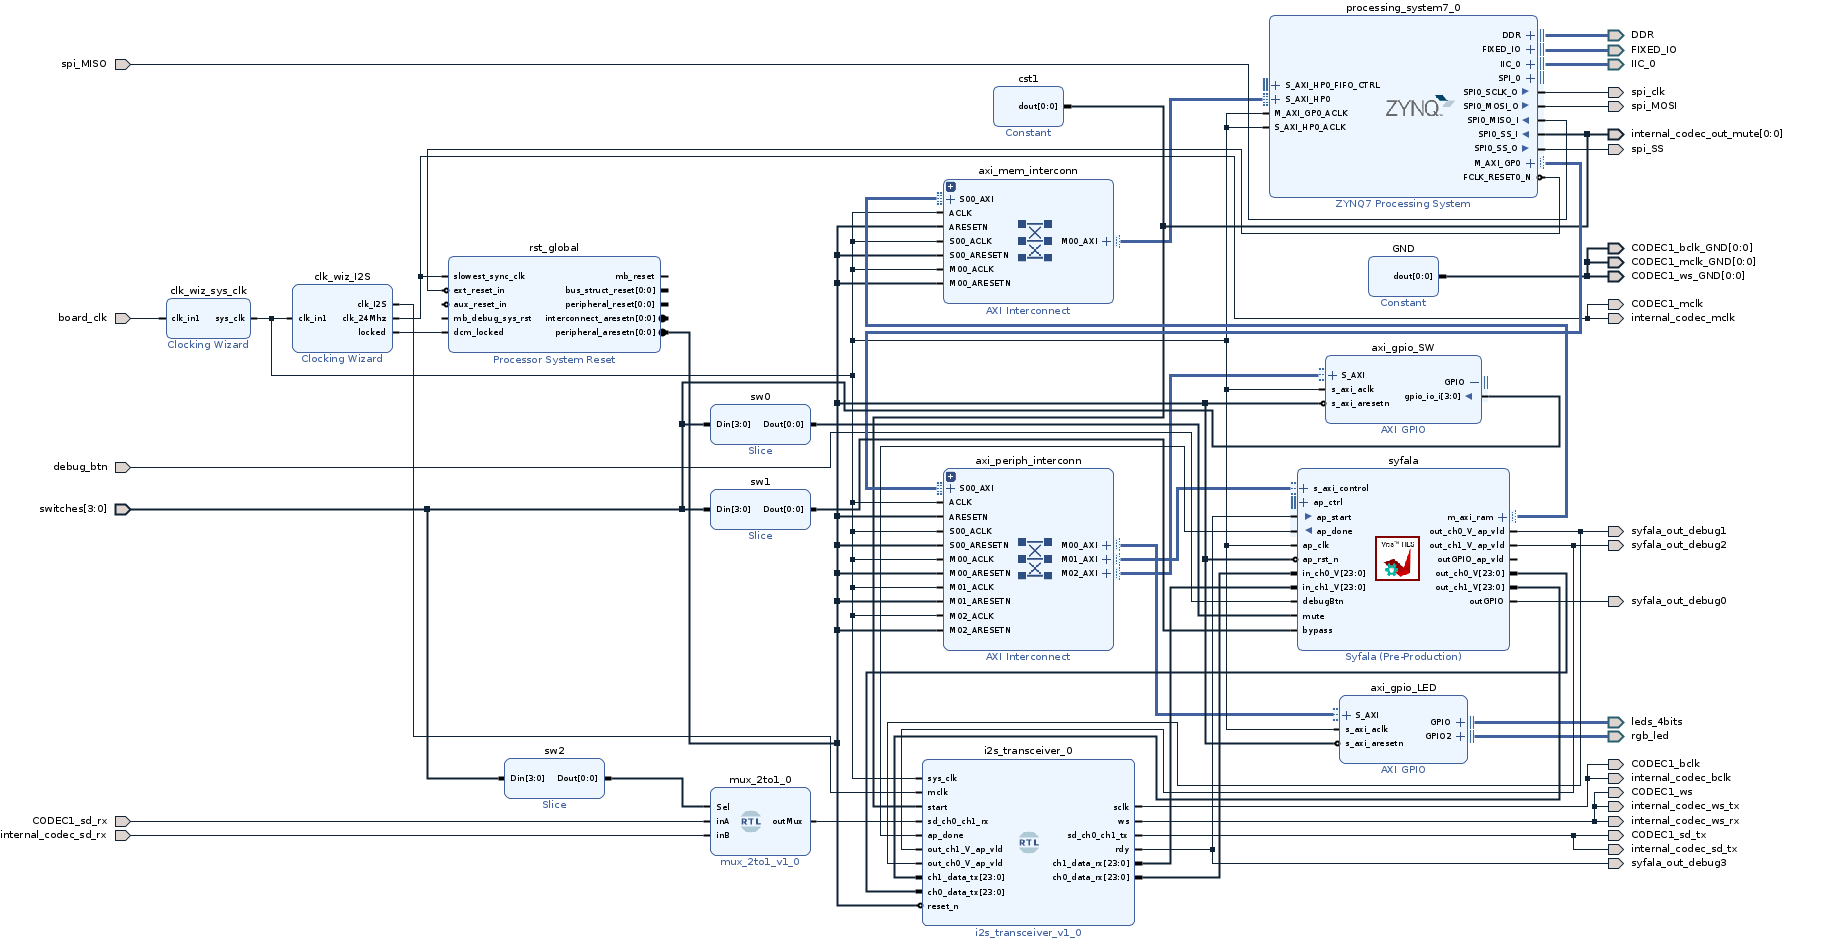
\includegraphics[width=16cm]{design_v7.png}}
  \caption{The bloc design obtained by connecting Syfala IP,(\syfala v7), with I2S IPs and AXI interface to DDR}
  \label{fig:design_6_3}
\end{figure}

Figure~\ref{fig:design_6_3} shows how the Faust IP, is interconnected with the rest of the system. All these IPs have a hardwired system clock at 122.88Mhz (i.e. approx. 8 ns system clock). It is very easy and very useful to open the {\tt vivado} project that generates the design. This can be done with the following command (after the build is done):
\begin{verbatim}
syfala open-project
\end{verbatim}\\
Then the  block design shown on Fig.~\ref{fig:design_6_3} can be opened using {\tt open Block Design}. One can see that the audio input/output streams of the Syfala IP are directly connected to the I2S IP ({\tt i2s\_transceiver} block), one can also see the {\tt AXI} IP interface which is used to access DDR and the {\tt axilite} IP interface used for interface with ARM processor.  The I2S IP is in turn directly connected to I/O of the Zynq with the following convention:
\begin{itemize}
\item The first two channels (Ch0 and Ch1) are connected to the pad of the onboard codec (SSM2603 for ZYBO, ADAU1761 for Genesys).
\item The first two channels (Ch0 and Ch1) are duplicated on GPIO pads for the use of an external codec.
\item All additional channels (if existing) are connected to the GPIO pads for the use of an external codec.
\end{itemize}
The onboard codec is configured from the ARM processor as described in section~\ref{sec:arm}\\



%\subsubsection{The {\tt i2s\_transceiver} IP}

%% \begin{figure}[ht]
%%   \centerline{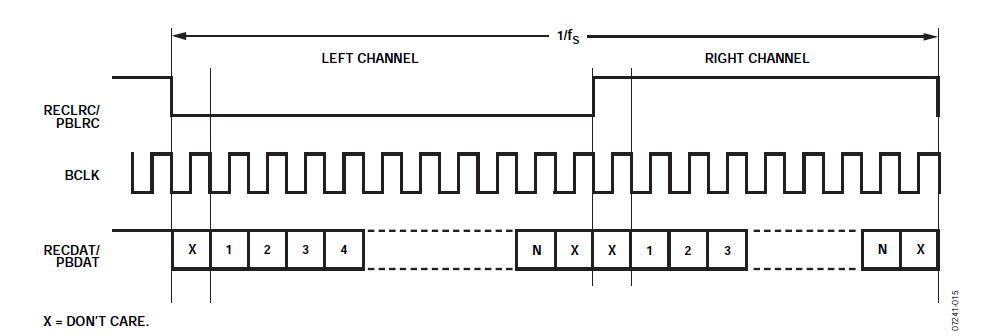
\includegraphics[width=\textwidth]{i2s_serialbit_mode.png}}
%%   \caption{J'ai laissé cette figure pour qu'on s'en inspire pour finit l'autre diagramme}
%%   \label{figi2sold}
%% \end{figure}


\begin{figure}[ht]
  \newcounter{wavenum}

\setlength{\unitlength}{1cm}
% advance clock one cycle, not to be called directly
\newcommand*{\clki}{
  \draw (t_cur) -- ++(0,-.3) -- ++(.2,0) -- ++(0,.6) -- ++(.2,0) -- ++(0,-.3)
    node[time] (t_cur) {};
}
%ws clock = 32 * clock
\newcommand*{\wsi}{
  \draw (t_cur) -- ++(0,.3) -- ++(6.4,0) -- ++(0,-.6) -- ++(6.4,0) -- ++(0,.6) -- ++(0.4,0)
    node[time] (t_cur) {};
}

\newcommand*{\bitvector}[3]{
  \draw[fill=#3] (t_cur) -- ++( .1, .3) -- ++(#2-.2,0) -- ++(.1, -.3)
                         -- ++(-.1,-.3) -- ++(.2-#2,0) -- cycle;
  \path (t_cur) -- node[anchor=mid] {#1} ++(#2,0) node[time] (t_cur) {};
}

% \known{val}{length}
\newcommand*{\known}[2]{
    \bitvector{{\tiny #1}}{#2}{white}
}

% \unknown{length}
\newcommand*{\unknown}[2][XXX]{
    \bitvector{{\tiny ..}}{#2}{black!2}
}

% \bit{1 or 0}{length}
\newcommand*{\bit}[2]{
  \draw (t_cur) -- ++(0,.6*#1-.3) -- ++(#2,0) -- ++(0,.3-.6*#1)
    node[time] (t_cur) {};
}

% \unknownbit{length}
\newcommand*{\unknownbit}[1]{
  \draw[ultra thick,black!50] (t_cur) -- ++(#1,0) node[time] (t_cur) {};
}
% \nextwave{name}
\newcommand{\nextwave}[1]{
  \path (0,\value{wavenum}) node[left] {#1} node[time] (t_cur) {};
  \addtocounter{wavenum}{-1}
}

% \clk{name}{period}
\newcommand{\clk}[2]{
    \nextwave{#1}
    \FPeval{\res}{(\wavewidth+1)/#2}
    \FPeval{\reshalf}{#2/2}
    \foreach \t in {1,2,...,\res}{
        \bit{\reshalf}{1}
        \bit{\reshalf}{0}
    }
}

% \ws{name}{period}
\newcommand{\ws}[2]{
    \nextwave{#1}
    \FPeval{\res}{(\wavewidth+1)/#2}
    \FPeval{\reshalf}{#2/2}
    \foreach \t in {1,2,...,\res}{
        \bit{\reshalf}{1}
        \bit{\reshalf}{0}
    }
}

% \begin{wave}[clkname]{num_waves}{clock_cycles}
\newenvironment{wave}[3][bclk]{
  \begin{tikzpicture}[draw=black, yscale=.7,xscale=1]
    \tikzstyle{time}=[coordinate]
    \setlength{\unitlength}{1cm}
    \def\wavewidth{#3}
    \setcounter{wavenum}{0}
    \nextwave{#1}
    \foreach \t in {0,1,...,\wavewidth}{
      \draw[dotted] (t_cur) +(0,.5) node[above] {{\tiny \t}} -- ++(0,.4-#2);
      \clki
      }
    \nextwave{ws}
    \wsi
}{\end{tikzpicture}}

\begin{wave}{2}{32}
  \nextwave{{ sd\_tx}}
  \known{x}{.4} \known{1}{.4} \known{2}{.4}
  \unknown[ ]{.4} \unknown[ ]{.4} \unknown[ ]{.4} \unknown[ ]{.4} \unknown[ ]{.4}\unknown[ ]{.4} \unknown[ ]{.4} \unknown[ ]{.4} \unknown[ ]{.4} \unknown[ ]{.4} \known{13}{.4} \known{14}{.4} \known{15}{.4} \known{16}{.4}
 \known{1}{.4} \known{2}{.4} \known{3}{.4} \known{4}{.4}
  \unknown[ ]{.4} \unknown[ ]{.4} \unknown[ ]{.4} \unknown[ ]{.4} \unknown[ ]{.4}\unknown[ ]{.4} \unknown[ ]{.4} \unknown[ ]{.4} \unknown[ ]{.4} \unknown[ ]{.4} \known{15}{.4} \known{16}{.4} 
  
\end{wave}

  \caption{I2S  protocol implemented {\tt i2s\_transceiver.vhd}, between the Syfala IP and  the audio codec with 16-bit samples. The {\tt ws} signal select from left or right channel. The {\tt  sd\_tx} bit stream corresponds to the 16 bits of the sample. it is shifted of 1 clock cycle from {\tt ws} changes. {\tt bclk} stands for {\em bit clock} and {\tt ws} stands for {\em word select}.}
  \label{figi2s}
\end{figure}

\begin{figure}[ht]
  \setlength{\unitlength}{1cm}
%mclk
\newcommand*{\mclki}{
  \draw (t_cur) -- ++(0,.3) -- ++(0.25,0) -- ++(0,-.6) -- ++(0.25,0) -- ++(0,.3)
    node[time] (t_cur) {};
}


% advance clock one cycle, not to be called directly
\newcommand*{\clki}{
  \draw (t_cur) -- ++(0,-.3) -- ++(1,0) -- ++(0,.6) -- ++(1,0) -- ++(0,-.3)
    node[time] (t_cur) {};
}

%ws clock = 32 * clock
\newcommand*{\wsi}{
  \draw (t_cur) -- ++(0,.3) -- ++(14,0)
    node[time] (t_cur) {};
}
\newcommand*{\wsitx}{
  \draw (t_cur) +(0,-.3) -- ++(1,-.3) -- ++(0,.6) -- ++(13,0)
    node[time] (t_cur) {};
}
\newcommand*{\wsirx}{
  \draw (t_cur) +(0,-.3) -- ++(2,-.3) -- ++(0,.6) -- ++(12,0)
    node[time] (t_cur) {};
}

\newcommand*{\bitvector}[3]{
  \draw[fill=#3] (t_cur) -- ++( .1, .3) -- ++(#2-.2,0) -- ++(.1, -.3)
                         -- ++(-.1,-.3) -- ++(.2-#2,0) -- cycle;
  \path (t_cur) -- node[anchor=mid] {#1} ++(#2,0) node[time] (t_cur) {};
}

% \known{val}{length}
\newcommand*{\known}[2]{
    \bitvector{{\tiny #1}}{#2}{white}
}

% \unknown{length}
\newcommand*{\unknown}[2][XXX]{
    \bitvector{{\tiny ..}}{#2}{black!2}
}

% \bit{1 or 0}{length}
\newcommand*{\bit}[2]{
  \draw (t_cur) -- ++(0,.6*#1-.3) -- ++(#2,0) -- ++(0,.3-.6*#1)
    node[time] (t_cur) {};
}

% \unknownbit{length}
\newcommand*{\unknownbit}[1]{
  \draw[ultra thick,black!50] (t_cur) -- ++(#1,0) node[time] (t_cur) {};
}

% \nextwave{name}
\newcommand{\nextwave}[1]{
  \path (0,\value{wavenum}) node[left] {#1} node[time] (t_cur) {};
  \addtocounter{wavenum}{-1}
}

% \clk{name}{period}
\newcommand{\clk}[2]{
    \nextwave{#1}
    \FPeval{\res}{(\wavewidth+1)/#2}
    \FPeval{\reshalf}{#2/2}
    \foreach \t in {1,2,...,\res}{
        \bit{\reshalf}{1}
        \bit{\reshalf}{0}
    }
}

% \ws{name}{period}
\newcommand{\ws}[2]{
    \nextwave{#1}
    \FPeval{\res}{(\wavewidth+1)/#2}
    \FPeval{\reshalf}{#2/2}
    \foreach \t in {1,2,...,\res}{
        \bit{\reshalf}{1}
        \bit{\reshalf}{0}
    }
}

% \begin{wave}[clkname]{num_waves}{clock_cycles}
\newenvironment{wave}[3][bclk]{
  \begin{tikzpicture}[draw=black, yscale=.7,xscale=1,scale=0.8,every node/.style={scale=0.8}]
    \tikzstyle{time}=[coordinate]
    \setlength{\unitlength}{1cm}
    \def\wavewidth{#3}
    \setcounter{wavenum}{0}
    \nextwave{mclk}
    \foreach \t in {0,1,...,2\wavewidth}{
      \mclki
      }
    \draw[dotted] (t_cur) -- ++(1,0);
    \nextwave{bclk (sclk)}
    \foreach \t in {0,1,...,\wavewidth}{
      \draw[dotted] (t_cur) +(0,1.5) node[above] {{\tiny \t}} -- ++(0,.4-#2);
      \clki 
      }
    \draw[dotted] (t_cur) -- ++(1,0);
    \nextwave{ws}
    \wsi \draw[dotted] (t_cur) -- ++(1,0);
    \nextwave{ws\_tx}
    \wsitx
    \nextwave{ws\_rx}
    \wsirx
}{\end{tikzpicture}}

\begin{wave}{3}{6}
  \nextwave{{ sd\_tx}}
  \known{$Left^{i-1}(15)$}{2} \known{$Right^{i}(0)$}{2} \known{$Right^{i}(1)$}{2} \known{$Right^{i}(2)$}{2} \known{$Right^{i}(3)$}{2} \known{$Right^{i}(4)$}{2} \known{$Right^{i}(5)$}{2} \draw[dotted] (t_cur) -- ++(1,0);
  \nextwave{{ sd\_rx}}
      \draw (t_cur)  ++(0, .3) -- ++(.9,0) -- ++(.1, -.3);
      \draw (t_cur)  ++(0, -.3) -- ++(.9,0) -- ++(.1, .3);
  %                       -- ++(-.1,-.3) -- ++(.2-.5,0)   -- cycle;
  \path (t_cur) -- node[anchor=mid] {~} ++(1,0) node[time] (t_cur) {};
         \draw[dotted] (t_cur) +(0,3.7)  -- ++(0,0);
          \known{$Left^{i-1}(15)$}{2} \draw[dotted] (t_cur) +(0,3.7)  -- ++(0,0);
\known{$Right^{i}(0)$}{2} \draw[dotted] (t_cur) +(0,3.7)  -- ++(0,0);
\known{$Right^{i}(1)$}{2}  \draw[dotted] (t_cur) +(0,3.7)  -- ++(0,0);
\known{$Right^{i}(2)$}{2}  \draw[dotted] (t_cur) +(0,3.7)  -- ++(0,0);
\known{$Right^{i}(3)$}{2}  \draw[dotted] (t_cur) +(0,3.7)  -- ++(0,0);
\known{$Right^{i}(4)$}{2}  \draw[dotted] (t_cur) +(0,3.7)  -- ++(0,0);
\known{$Right^{i}(5)$}{2} \draw[dotted] (t_cur) -- ++(1,0);
\end{wave}

  \caption{Zoom on the beginning of a right sample  (sample number $i$) first bits transmission: {\tt mclk} is 4 time faster than {\tt bclk}. {\tt ws\_tx} and {\tt ws\_rx} are delayed version of {\tt ws}, used to synchronize starting of  samples bits transmission. {\tt sd\_tx} is {\em produced} by the I2S IP as an output on the falling edge of {\tt bclk} and {\tt sd\_rx} is {\em read} as an input on the rising edge of {\tt bclk}.}
  \label{figi2szoom1}
\end{figure}

The {\tt i2s\_transceiver} is the one that really transmits the bits between the FPGA and the audio codec. The data is serialized and transmitted/received on the {\tt sd\_tx}/{\tt sd\_rx} port to the ports of the audio codec. The protocol used in our design is the one illustrated on Fig.~\ref{figi2s}, it can be configured to send 16, 24 or 32 bit-wide sample. For 16 bit configuration the sample cycle time is exactly divided in 32 cycles to transmit the $2\times16$ bits (left and right samples), as shown on Fig.~\ref{figi2s}. But for 24 bit-wide sample, the sample cycle is not divided in 48 (=$2\times24$), but in 64 cycles as it is for 32  bit-wide samples.  The sample bits are serially transmitted along the {\tt bclk} clock as shown in Fig.~\ref{figi2s} (see also~\cite{ssm2603}). The {\tt ws} signal indicates whether current bits belong to  left or right channel. However, as indicated in Fig.~\ref{figi2s}, there is a shift of 1 cycle: the first bit send after {\tt ws} clock fall-down is not the first bit of current left sample, it is the last bit of the previous right sample.\footnote{See for instance \url{https://www.sparkfun.com/datasheets/BreakoutBoards/I2SBUS.pdf}}

\paragraph{Syfala I2S patch} In a normal transmission, the {\tt sd\_tx} bit is positioned on the falling edge of {\tt bclk} clock, it is transmitted from our (master) I2S to the (slave) I2S of the codec. Simultaneously, the slave I2S is positioning the {\tt sd\_rx} bit -- which is {\em his} {\tt sd\_tx} -- to be transmitted from the codec to our I2S. The {\tt sd\_rx} bit is effectively read by our I2S on the rising edge of {\tt bclk}, this allows time for the signal to arrive through the connection between the codec and the FPGA, this time is called {\tt Tsod} in analog device ADAUs codecs for instance (see Fig.~\ref{figi2szoom2}-(a) for illustration).  

In our design, we have used external codecs that allows internal clock as fast as 768kHz. We have noticed that, as we needed a level shifter to adapt power supplies between the codec and the Zybo, this  half a bclk cycle time may be less than the time needed for {\tt sd\_rx} to stabilize. Hence we proposed a {\em patch} that delays of one  {\tt mclk} cycle in addition to the half {\tt bclk} cycle shown on Fig.~\ref{figi2szoom2}-(b).

\begin{figure}[ht]
  \begin{tabular}{cc}
    \begin{boxedminipage}{0.5\textwidth}
      \def\decalage{.7}
\def\shift{.3}

\setlength{\unitlength}{1cm}
%mclk
\newcommand*{\mclki}{
  \draw (t_cur) -- ++(0,.3) -- ++(0.25,0) -- ++(0,-.6) -- ++(0.25,0) -- ++(0,.3)
    node[time] (t_cur) {};
}


% advance clock one cycle, not to be called directly
\newcommand*{\clki}{
  \draw (t_cur) -- ++(0,-.3) -- ++(1,0) -- ++(0,.6) node[time] (t_cur) {};
  \draw[dotted] (t_cur) +(0,-3.7)  -- ++(0,0);
  \draw (t_cur)  -- ++(1,0) -- ++(0,-.3)    node[time] (t_cur) {};
}

%ws clock = 32 * clock
\newcommand*{\wsi}{
  \draw (t_cur) -- ++(0,.3) -- ++(14,0)
    node[time] (t_cur) {};
}
\newcommand*{\wsil}{
  \draw (t_cur) +(0,-.3) -- ++(2,-.3) -- ++(0,.6) -- ++(12,0)
    node[time] (t_cur) {};
}

\newcommand*{\bitvector}[3]{
  \draw[fill=#3] (t_cur) -- ++( .1, .3) -- ++(#2-.2,0) -- ++(.1, -.3)
                         -- ++(-.1,-.3) -- ++(.2-#2,0) -- cycle;
  \path (t_cur) -- node[anchor=mid] {#1} ++(#2,0) node[time] (t_cur) {};
}

% \known{val}{length}
\newcommand*{\known}[2]{
    \bitvector{{\tiny #1}}{#2}{white}
}

% \unknown{length}
\newcommand*{\unknown}[2][XXX]{
    \bitvector{{\tiny ..}}{#2}{black!2}
}

% \bit{1 or 0}{length}
\newcommand*{\bit}[2]{
  \draw (t_cur) -- ++(0,.6*#1-.3) -- ++(#2,0) -- ++(0,.3-.6*#1)
    node[time] (t_cur) {};
}

% \unknownbit{length}
\newcommand*{\unknownbit}[1]{
  \draw[ultra thick,black!50] (t_cur) -- ++(#1,0) node[time] (t_cur) {};
}

% \nextwave{name}
\newcommand{\nextwave}[1]{
  \path (0,\value{wavenum}) node[left] {#1} node[time] (t_cur) {};
  \addtocounter{wavenum}{-1}
}

% \clk{name}{period}
\newcommand{\clk}[2]{
    \nextwave{#1}
    \FPeval{\res}{(\wavewidth+1)/#2}
    \FPeval{\reshalf}{#2/2}
    \foreach \t in {1,2,...,\res}{
        \bit{\reshalf}{1}
        \bit{\reshalf}{0}
    }
}

% \ws{name}{period}
\newcommand{\ws}[2]{
    \nextwave{#1}
    \FPeval{\res}{(\wavewidth+1)/#2}
    \FPeval{\reshalf}{#2/2}
    \foreach \t in {1,2,...,\res}{
        \bit{\reshalf}{1}
        \bit{\reshalf}{0}
    }
}

% \begin{wave}[clkname]{num_waves}{clock_cycles}
\newenvironment{wave}[3][bclk]{
  \begin{tikzpicture}[draw=black, yscale=.7,xscale=1,scale=0.8,every node/.style={scale=0.8}]
    \tikzstyle{time}=[coordinate]
    \setlength{\unitlength}{1cm}
    \setcounter{wavenum}{0}
    \nextwave{mclk}
    \foreach \t in {0,1,...,12}{
      \mclki
      }
    \draw[dotted] (t_cur) -- ++(1,0);
    \nextwave{bclk}
    \foreach \t in {0,1,...,2}{
      \draw[dotted] (t_cur) +(0,1.5) node[above] {{\tiny \t}} -- ++(0,.4-#2);
      \clki 
      }
    \draw[dotted] (t_cur) -- ++(1,0);
}{\end{tikzpicture}}

\begin{wave}{3}{3}
  \nextwave{{ sd\_tx}}
  \known{$Left^{i-1}(15)$}{2} \known{$Right^{i}(0)$}{2} \known{$Right^{i}(1)$}{2} -- ++(1,0);
  \nextwave{~}
  \draw[very thick] (t_cur) ++(0, 0.3) -- ++(0,-.6);
  \draw[very thick] (t_cur) ++(\decalage, .3) -- ++(0,-1.2);
  \draw[<->,thick] (t_cur)++(0,0)  --  node[below] {\tiny $T_{sod}$} ++(\decalage,0);
  \nextwave{{ sd\_rx}}
      \draw (t_cur)  ++(0, .3) -- ++(\decalage+\shift-.1,0) -- ++(.1, -.3);
      \draw (t_cur)  ++(0, -.3) -- ++(\decalage+\shift-.1,0) -- ++(.1, .3);
  %                       -- ++(-.1,-.3) -- ++(.2-.5,0)   -- cycle;
  \path (t_cur) -- node[anchor=mid] {~} ++(\decalage+\shift,0) node[time] (t_cur) {};
  \known{$Left^{i-1}(15)$}{2} %\draw[dotted] (t_cur) +(0,3.7)  -- ++(0,0);
\known{$Right^{i}(0)$}{2} %\draw[dotted] (t_cur) +(0,3.7)  -- ++(0,0);
\known{$Right^{i}(1)$}{2}  %\draw[dotted] (t_cur) +(0,3.7)  -- ++(0,3.7);
\end{wave}

      \end{boxedminipage} &
    \begin{boxedminipage}{0.5\textwidth}
      \def\decalage{.7}
\def\shift{.8}

\setlength{\unitlength}{1cm}
%mclk
\newcommand*{\mclki}{
  \draw (t_cur) -- ++(0,.3) -- ++(0.25,0) -- ++(0,-.6) -- ++(0.25,0) -- ++(0,.3)
    node[time] (t_cur) {};
}


% advance clock one cycle, not to be called directly
\newcommand*{\clki}{
  \draw (t_cur) -- ++(0,-.3) -- ++(1,0) -- ++(0,.6) node[time] (t_cur) {};
  \draw[dotted] (t_cur) +(0.5,-3.7)  -- ++(0.5,0.4);
  \draw (t_cur)  -- ++(1,0) -- ++(0,-.3)    node[time] (t_cur) {};
}

%ws clock = 32 * clock
\newcommand*{\wsi}{
  \draw (t_cur) -- ++(0,.3) -- ++(14,0)
    node[time] (t_cur) {};
}
\newcommand*{\wsil}{
  \draw (t_cur) +(0,-.3) -- ++(2,-.3) -- ++(0,.6) -- ++(12,0)
    node[time] (t_cur) {};
}

\newcommand*{\bitvector}[3]{
  \draw[fill=#3] (t_cur) -- ++( .1, .3) -- ++(#2-.2,0) -- ++(.1, -.3)
                         -- ++(-.1,-.3) -- ++(.2-#2,0) -- cycle;
  \path (t_cur) -- node[anchor=mid] {#1} ++(#2,0) node[time] (t_cur) {};
}

% \known{val}{length}
\newcommand*{\known}[2]{
    \bitvector{{\tiny #1}}{#2}{white}
}

% \unknown{length}
\newcommand*{\unknown}[2][XXX]{
    \bitvector{{\tiny ..}}{#2}{black!2}
}

% \bit{1 or 0}{length}
\newcommand*{\bit}[2]{
  \draw (t_cur) -- ++(0,.6*#1-.3) -- ++(#2,0) -- ++(0,.3-.6*#1)
    node[time] (t_cur) {};
}

% \unknownbit{length}
\newcommand*{\unknownbit}[1]{
  \draw[ultra thick,black!50] (t_cur) -- ++(#1,0) node[time] (t_cur) {};
}

% \nextwave{name}
\newcommand{\nextwave}[1]{
  \path (0,\value{wavenum}) node[left] {#1} node[time] (t_cur) {};
  \addtocounter{wavenum}{-1}
}

% \clk{name}{period}
\newcommand{\clk}[2]{
    \nextwave{#1}
    \FPeval{\res}{(\wavewidth+1)/#2}
    \FPeval{\reshalf}{#2/2}
    \foreach \t in {1,2,...,\res}{
        \bit{\reshalf}{1}
        \bit{\reshalf}{0}
    }
}

% \ws{name}{period}
\newcommand{\ws}[2]{
    \nextwave{#1}
    \FPeval{\res}{(\wavewidth+1)/#2}
    \FPeval{\reshalf}{#2/2}
    \foreach \t in {1,2,...,\res}{
        \bit{\reshalf}{1}
        \bit{\reshalf}{0}
    }
}

% \begin{wave}[clkname]{num_waves}{clock_cycles}
\newenvironment{wave}[3][bclk]{
  \begin{tikzpicture}[draw=black, yscale=.7,xscale=1,scale=0.8,every node/.style={scale=0.8}]
    \tikzstyle{time}=[coordinate]
    \setlength{\unitlength}{1cm}
    \setcounter{wavenum}{0}
    \nextwave{mclk}
    \foreach \t in {0,1,...,12}{
      \mclki
      }
    \draw[dotted] (t_cur) -- ++(1,0);
    \nextwave{bclk}
    \foreach \t in {0,1,...,2}{
      \draw[dotted] (t_cur) +(0,1.5) node[above] {{\tiny \t}} -- ++(0,.4-#2);
      \clki 
      }
    \draw[dotted] (t_cur) -- ++(1,0);
}{\end{tikzpicture}}

\begin{wave}{3}{3}
  \nextwave{{ sd\_tx}}
  \known{$Left^{i-1}(15)$}{2} \known{$Right^{i}(0)$}{2} \known{$Right^{i}(1)$}{2} -- ++(1,0);
  \nextwave{~}
  \draw[very thick] (t_cur) ++(0, 0.3) -- ++(0,-.6);
  \draw[very thick] (t_cur) ++(\decalage, .3) -- ++(0,-.6);
  \draw[<->,thick] (t_cur)++(0,0)  --  node[below] {\tiny $T_{sod}$} ++(\decalage,0) node[time] (t_cur) {};
  
  \draw[very thick] (t_cur) ++(\shift, .3) -- ++(0,-1.2);
  \draw[<->,thick] (t_cur)++(0,0)  --  node[above,yshift=0.2] {\tiny $^{shifter}$} ++(\shift,0);
  \nextwave{{ sd\_rx}}
      \draw (t_cur)  ++(0, .3) -- ++(\decalage+\shift-.1,0) -- ++(.1, -.3);
      \draw (t_cur)  ++(0, -.3) -- ++(\decalage+\shift-.1,0) -- ++(.1, .3);
  %                       -- ++(-.1,-.3) -- ++(.2-.5,0)   -- cycle;
  \path (t_cur) -- node[anchor=mid] {~} ++(\decalage+\shift,0) node[time] (t_cur) {};
  \known{$Left^{i-1}(15)$}{2} %\draw[dotted] (t_cur) +(0,3.7)  -- ++(0,0);
\known{$Right^{i}(0)$}{2} %\draw[dotted] (t_cur) +(0,3.7)  -- ++(0,0);
\known{$Right^{i}(1)$}{2}  %\draw[dotted] (t_cur) +(0,3.7)  -- ++(0,3.7);
\end{wave}

            \end{boxedminipage}\\
  (a) Standard I2S & (b) Patched I2S \\
  \end{tabular}
  \caption{The left chronogram (a) illustrates the {\tt Tsod} time needed for the information to transit from codec to FPGA. In a standard I2S, the {\tt sd\_rx} bit is sampled on the rising edge of {\tt bclk}. On the right (b) is illustrated our patch delaying the sampling of a {\tt mclk} period, taking into account the time needed to transit through the level shifter}
  \label{figi2szoom2}
\end{figure}

We have implemented the I2S protocol in VHDL (file {\tt src/i2s\_transceiver.vhd}). It can be parameterized by the  sample bit depth as well as by the sample rate.  

The {\tt i2s\_transceiver} is connected to the {\tt Syfala} IP. It performs a hand shake ({\tt ap\_hs} protocol from Xilinx {\tt vitis\_hls}) with the Syfala IP in order to transmit and receive samples from the Syfala IP. The {\tt ap\_start} signal is initiated by the {\tt i2s\_transceiver} and when the two Syfala IP outputs are ready ({\tt out\_ch0\_V} and {\tt out\_ch1\_V}), the signals {\tt out\_ch0\_V\_ap\_vld} and {\tt out\_ch1\_V\_ap\_vld} are raised {\em for one system clock cycle}. A hand shake is proposed in the I2S transceiver to grab the output values when they are available (they are not necessarily available simultaneously). 


\subsection{Time, Clocks and the ordering of ticks in the Syfala system}

It is important to understand the origin and value of the different clocks in the system. The generation of the different clocks is highly simplified by the use of two {\tt Clocking Wizard} IP. The first clocking wizard  inputs the  external clock ({\tt sys\_clk}) and outputs the FPGA system clock {\tt board\_clk} and the second one outputs {\tt mclk} and another clock at 24MHz needed by the codecs. The reason for using {\em two} clocking wizard instead of one is that exact frequencies for the three clocks cannot be obtained with only one clocking wizard, we need two MMCM/PLL.   

\paragraph{FPGA system Clock: {\tt sys\_clk} at 122.88MHz}
The {\em internal} FPGA clock that triggers every registers of the FPGA is depending of the complexity of the design (i.e. the complexity of the longest combinatorial path), it is called {\tt sys\_clk} on Vivado block design. We follow two rules to set this clock:
\begin{itemize}
\item {\tt sys\_clk} can be as fast as wanted as long as it met timing constraints.
\item  {\tt sys\_clk} and {\tt mclk} should be multiples to facilitate the timing closure and minimize the negative slack.
\end{itemize}
{\tt mclk} is a multiple of 48kHz and $f_{mclk}$=12.288MHz at 48kHz sampling rate (see below). So we usually impose {\tt sys\_clk} clock to be {\bf 122.88MHz} (i.e. setting  a {\bf 8.13ns} clock when creating {\tt vivado} and {\tt vivado\_hls} projects). Faster clocks have been tested with Syfala and should work too.

\paragraph{I2S Transceiver Master Clock: {\tt clk\_I2S} at $ 2\times 4 \times d_{width}\times f_s$}
We call $d_{width}$ the number of cycle needed to send the bits of one sample,  remember that, as explained above: $d_{width}$ is 16 for 16 bit-wide samples but 32 for 24 bit wide samples (and 32 for 32 bit wide samples too).   
The clock regulating the transceiver ({\tt mclk}) should be a multiple of the sampling frequency, it should be exactly $f_{mclk}=2\times 4\times d_{width}\times f_s$, where $f_s$ is the sample rate. Indeed, as $bclk$ clock will be four times  slower than $mclk$ clock, we will have time to send 2 samples of $d_{width}$ bits in one sample cycle. 

For instance, if we want an I2S signal at 48kHz sampling rate with 24 bit samples, $f_{mclk}$ should be: $$f_{mclk}=8 \times 32 \times f_s=256*48kHz =12.288MHz$$

\paragraph{Codec system clock: {\tt clk\_24Mhz} at 24.576MHz} The last generated clock is the system clock needed by the codecs to works. It's configurable on each codec and has no effect on the sampling rate. We use a {\bf 24.576MHz} clock which is compatible with all our tested codecs and ensure the best performances.\\

{\em In practice, the clocking wizard is not able to obtain exactly the these frequencies (because of the limitation of a PLL) so the real sample frequency obtained is not exactly 48kHz. But we ensure that all frequencies are multiples specifying the nearest synthesizable frequency. For exemple, on ZYBO we have:}
$f_{sys\_clk}$=122.885835MHz, $f_{clk\_I2S}$=12.2885835MHz so $f_{s}$=48.002279kHz

\paragraph{The {\tt i2s\_transceiver} clocks}
The I2S transceiver is using two more clocks: the {\bf sclk} clock, sometimes called  {\bf bclk} ({\em bit clock} because it is clocking each bit as illustrated on figure~\ref{figi2s}) and the {\bf ws} clock (word select) which select the left or right channel (illustrated as {\tt ws} on Fig.~\ref{figi2s}).

There is a fixed ratio between these two clocks and the {\tt mclk} mentioned above:{\tt mclk/sclk}=4 (i.e. {\tt mclk} is 4 time faster {\tt sclk}). The ratio between {\tt sclk} and {\tt ws} is also fixed but it depends on the bit depth of the sample: {\tt sclk/ws}$=2\times d_{width}$. We have hard-coded these ratios  in {\tt i2s\_transceiver.vhd} generic VHDL parameters which are generated at compile time, depending on the sample bit-depth given as options to the {\tt syfala} command (24 by default).

For instance, at  48kHz sampling rate with 24 bit samples,  one {\tt ws} period is $T_{ws}=4\times 2\times 32\times T_{mclk}=256\times T_{mclk}=T_{audio}=\frac{1}{48kHz}=20.83\mu s$. Here are the generic parameters used for this configuration in {\tt i2s\_transceiver.vhd}

{\small
\begin{verbatim}
  generic(
    mclk_sclk_ratio : integer := 4;   --number of mclk periods per sclk period
    sclk_ws_ratio   : integer := 64;  --number of sclk periods per word select period
    d_width         : integer := 24); --data width
\end{verbatim}
}


\begin{figure}[ht]
  \centerline{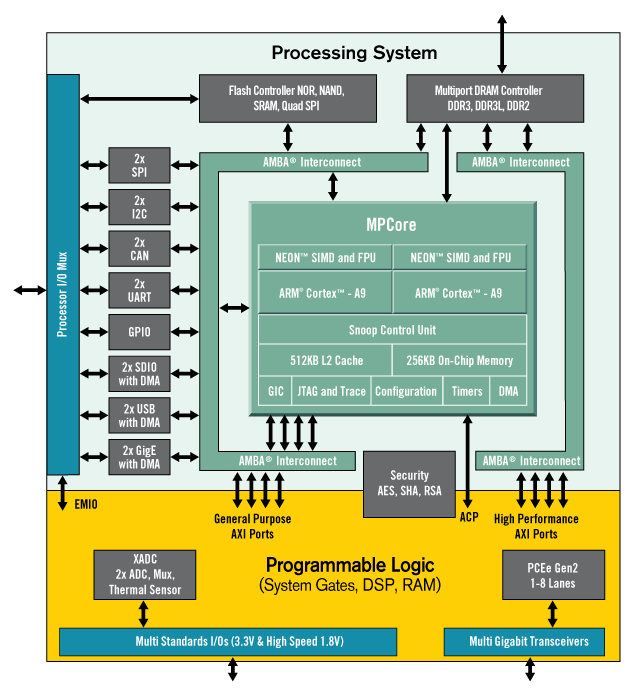
\includegraphics[width=7cm]{zynq-mp-core-dual1.png}}
  \caption{Architecture of Xilinx Zynq 7000 (ZYBO) processing system (from \url{https://www.xilinx.com/products/silicon-devices/soc/zynq-7000.html})}
  \label{zynq}
\end{figure}

\begin{figure}[ht]
  \centerline{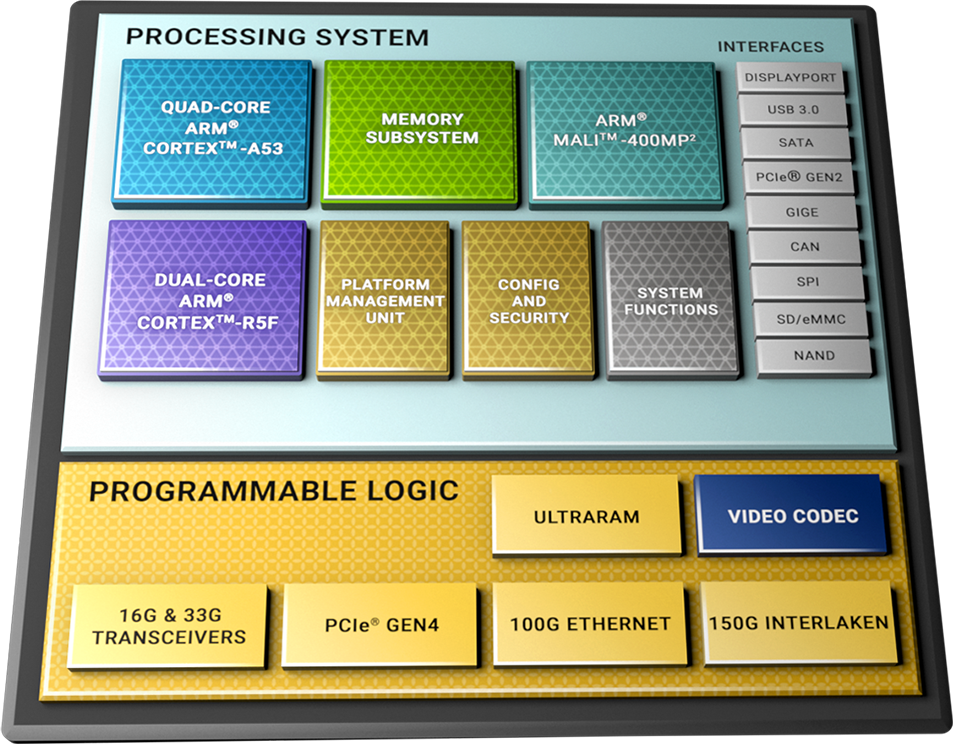
\includegraphics[width=7cm]{fig/ultrascale_MPSOC.png}}
  \caption{Architecture of Xilinx UltraScale+ (Genesys) processing system (from \url{https://www.xilinx.com/products/silicon-devices/soc/zynq-ultrascale-mpsoc.html})}
  \label{ultrascale}
\end{figure}
\subsection{The ARM application software  and the {\tt arm.cpp} architecture file}
\label{sec:arm}


Zynq SoCs include a so-called {\em processing system} which consists in a
 dual-core ARM Cortex-A9 for Zynq7000 SoC for ZYBO, or a Quad-core ARM Cortex-A53 on Ultrascale+ MPSoC for Genesys ZU-3EG.
These SoC also embed a high performance and general purpose buses between ARM and FPGA (axilite port) and an interface to an external DDR memory (see Fig.~\ref{zynq} and Fig.~\ref{ultrascale}). 

Ideally, the DSP computations should be executed on the FPGA and the control and initialization should be executed on  the ARM processor.  The Faust language proposes several interfaces to the user: sliders or button and even feedback information. In the remaining of this documents, we will refer to these interface devices as {\em controllers}.

The {\tt faust}  compiler is invoked a second time. The first invocation  has generated the {\tt syfala.cpp} file used to generate the IP (using the {\tt fpga.cpp} architecture file). The second invocation is used to generate the {\tt syfala\_application.cpp} program that will run on the ARM (using the {\tt arm.cpp} architecture file).


The   {\tt syfala\_application.cpp} is quite long because it re-uses many contributions from the Faust ecosystem. Here are the actions executed by the application on the ARM processor (i.e. the actions of the {\tt syfala\_application.cpp} file):
  \begin{itemize}
  \item It initializes the {\tt ddr\_ptr} pointer to the DDR memory and erases the part of the memory used by the FPGA IP. The address of the {\tt ddr\_ptr} is  inherited from a macro defined in the linker script: 
\begin{verbatim}
    u32* ddr_ptr = (u32*)FRAME_BUFFER_BASEADDR;
\end{verbatim}

\item It initializes the {\tt izone} and {\tt fzone} which are then transmitted to the Faust IP:
\begin{verbatim}
        iZone = (int*)(ddr_ptr);
        fZone = (float*)(ddr_ptr + FAUST_INT_ZONE);
\end{verbatim}
\item It initializes various peripherals of the Soc:
  \begin{itemize}
  \item GPIOs
  \item SPI peripheral (used to get controlers/sliders valuers)
  \item I2C (used to configure the audio codec)
  \item Faust IP
  \item DDR memory
  \end{itemize}
\item It defines a user interface for the DSP program ({\tt UI})
\item It defines a class {\tt mydsp} which correspond to all the variables of the DSP program  stored in the Block Rams by the Faust IP: delay lines, temporary computation, etc. This ``additional'' declaration is used to initialize some of these variables (in particular constants).
  \item It maintains a state for each controller and updates them when their values changes, either from hardware (in case of hardware interface) or from software (i.e. via the UART connection in case of software interface).
  \item It sends these controllers values repetitively to the Faust IP.
  \end{itemize}
\begin{figure}[ht]
\centering
  \begin{tabular}{ccc}
    %knob: piqué sur internet: https://tex.stackexchange.com/questions/525535/creating-a-audio-volume-dial-using-tikz
\def\centerarc[#1](#2)(#3:#4:#5)
              { \draw[#1] ($(#2)+({#5*cos(#3)},{#5*sin(#3)})$) arc (#3:#4:#5); }


\newcommand\knob[1]{
\centerarc[name path=arcc,fill=none,draw=black,line width=0.2]($(#1)$)(-60:240:2mm)
%\foreach \t [count=\i from 0] in {-60,-30,...,240}{
\foreach \t [count=\i from 0] in {240,210,...,-60}{
\path [name path=\t]($(#1)$)--++(\t:8.2mm);
\path [name intersections={of=arcc and \t,by={\t1}}];
\draw [line cap=round, line width=0.2](\t1)--++(\t:0.5mm);
\path (\t1)--++(\t:1.5mm)node{\scalebox{0.5}{$\i$}};
}
}

\begin{tikzpicture}[>=stealth']
  \node[draw=black,minimum height=1cm] (arm) {ARM};
  \node[draw=black, below of=arm,minimum width=1.5cm, yshift=-0.4cm] (ip) {Faust IP};
  \node[draw=black,left of=arm, xshift=-0.5cm,rounded rectangle](type){\tiny HW/SW ?};
  \node[draw=black, fit=(arm)(ip)(type),minimum height=1.5cm,minimum width=1.5cm][thick] (zybo) {};

  \node[draw=black,yshift=1cm,xshift=-0.5cm,minimum width=2.5cm,minimum height=1cm,left=of zybo,label={[xshift=-0.5cm,yshift=-0.1cm]\tiny Controller Board}] (interfBoard) {};
  \knob{$(interfBoard)+(-0.5cm,0cm)$};
  \knob{$(interfBoard)+(0.5cm,0cm)$};
  \node[draw=black,inner sep=0pt,minimum width=2.5cm,minimum height=1.5cm,below of=interfBoard,  yshift=-0.7cm,label={[xshift=-0.8cm,yshift=-0.1cm]\tiny Host PC}] (hostPC) {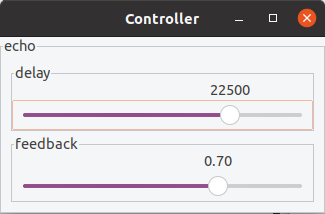
\includegraphics[width=2.5cm]{gtkUI.png}};
  
  \node[right of=hostPC,yshift=0.15cm,xshift=1cm] (uart) {\tiny UART/USB};
  \node[right of=interfBoard,yshift=0.15cm,xshift=0.6cm] (spi) {\tiny SPI};


 \draw[<-][thick] (ip) -- node[right]{\footnotesize s-AXI} (arm);
 \draw[->][thick] (type) -- (arm);
 \draw[->][thick] (hostPC) --++(100pt,0pt) --++(0pt,30pt);
 \draw[->][thick] (interfBoard) --++(100pt,0pt) --++(0pt,-6pt);

\end{tikzpicture}

&~~~~ &
    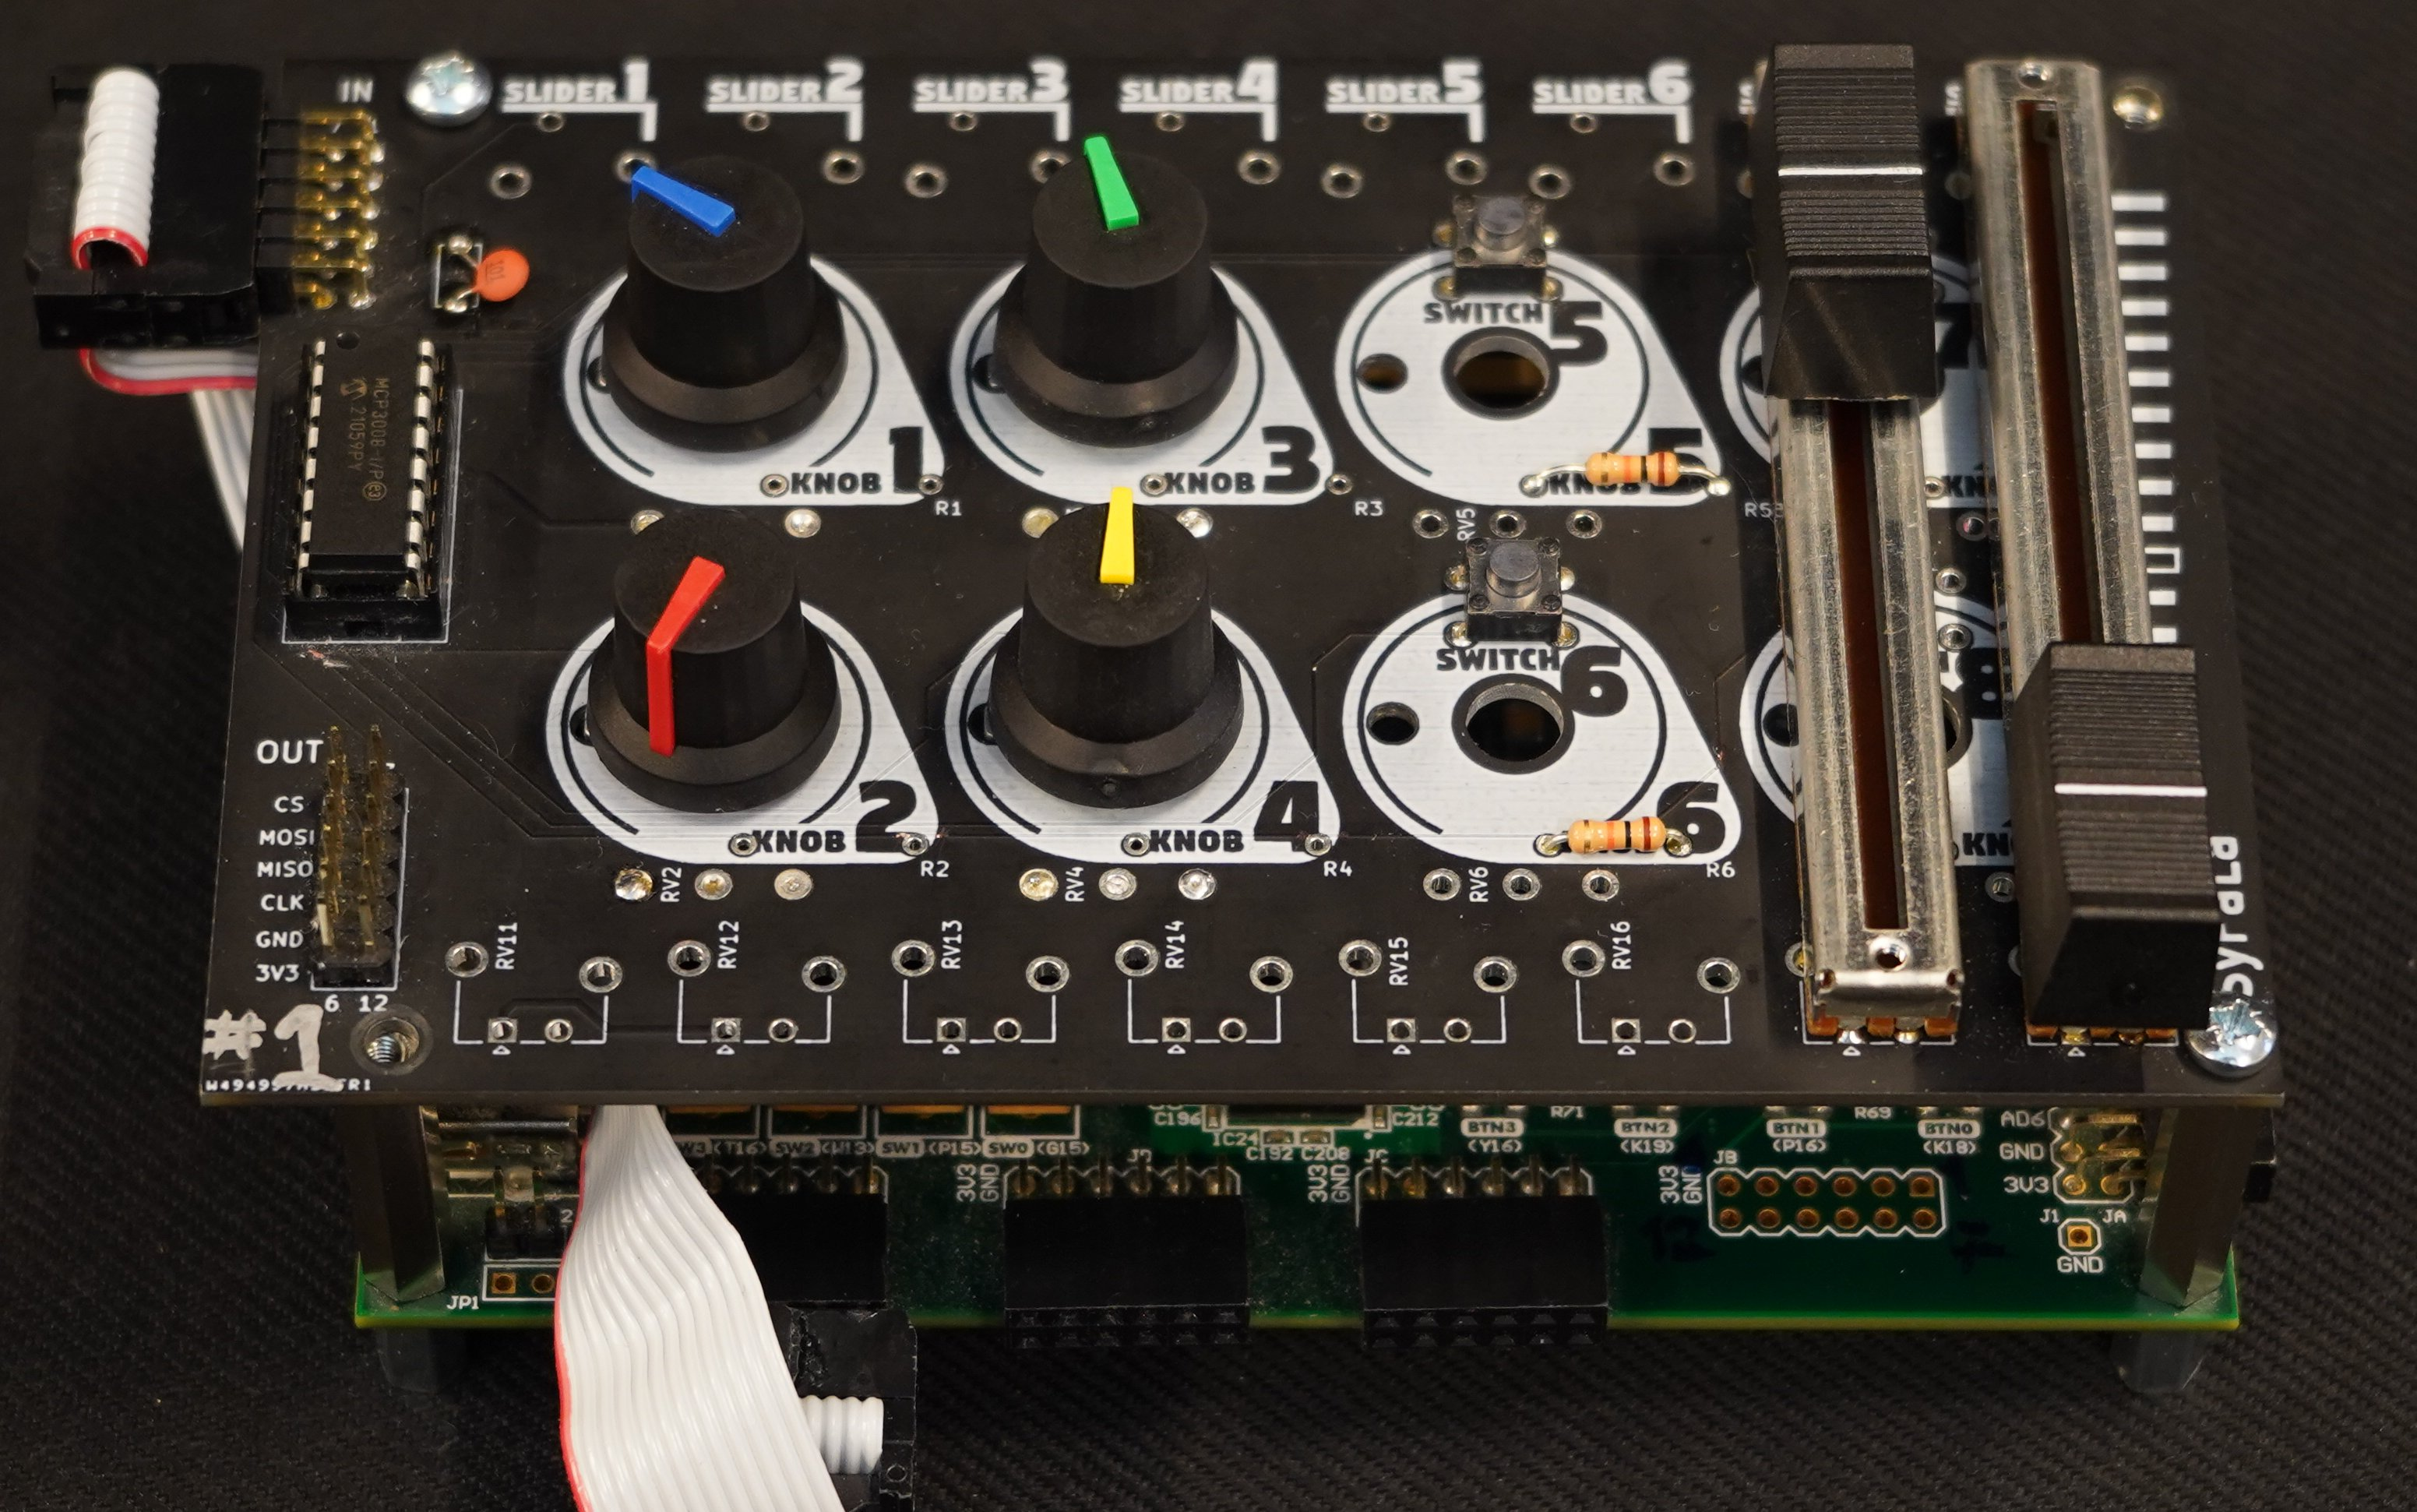
\includegraphics[width=4cm]{fig/popophone.jpg}\\
    (a) & &(b)
    \end{tabular}
\caption{(a) Interface selection between software interface (GTK app) and hardware interface (knobs such those shown in (b)). The design of the hardware board such as (b) can be freely available on github.}
\label{fig:interfaceOverview}
\end{figure}
  The {\tt syfala\_application.elf} file is cross-compiled to ARM binary format on the host using the cross compilation tool proposed by {\tt vitis} from the files {\tt syfala\_application.cpp}, and some other files present in the {\tt src} directory. The compilation is configured by Xilinx {\tt xsct} tool using the script {\tt scripts/application.tcl}

Depending on the information of the syfala command, the code executed by {\tt syfala\_application.elf} launches a hardware interface to control the Faust IP or a software interface to control the Faust IP. This is shown on Fig.~\ref{fig:interfaceOverview}.


\section{A complete example: simple sinewave}
\label{example}
\label{sec:example}
Imagine we want to implement on FPGA a filter-based sine wave oscillator. Such a sine wave is written in Faust in Fig.~\ref{fig:osc}, it is available in Syfala repository as program {\tt sinewave-biquad-inlined.dsp} of the {\tt examples} directory. There is one controller which selects the oscillator frequency. Note the {\tt ``[knob:1]''} meta data that indicates that this controller will be associated to the first knob in case of hardware interface.

The computation of {\tt th}, {\tt c} and {\tt s} are depending on the frequency value, hence we expect all these variables to be computed at control rate, hence on the ARM, not on the FPGA. On the other hand, the computation of {\tt nlf2} is performed at each sample (sample rate) and will be implemented on the FPGA.


\begin{figure}[ht]
  \begin{boxedminipage}{\columnwidth}
    \tiny
    \verbatiminput{fig/sinewave-biquad-inlined.dsp}
  \end{boxedminipage}
  \caption{Filter-based sine wave oscillator in Faust used for illustrating the compilation process (file {\tt sinewave-biquad-inlined.dsp} in {\tt examples} directory).}
  \label{fig:osc}
  \label{fig:biquad}
\end{figure}

The whole compilation can be done using the command:\\
{\tt syfala examples/sinewave-biquad-inlined.dsp}\\
but we will detail the different steps.

The first step of the compilation flow is to generate a C++ program from the Faust code, this is done by executing:\\
\verb#syfala examples/sinewave-biquad-inlined.dsp --arch --reset# \\
this command will generate {\tt syfala\_ip.cpp} and {\tt syfala\_application.cpp} files. All the generated files  are generated in the directory {\tt build/}. The \verb#--reset# options is mandatory if another project has already been compiled in the {\tt build} directory. Warning, the \verb#--reset# option will erase your previous compiled Syfala project.

The \verb#--arch# option generates the {\tt syfala\_ip.cpp} file in directory {\tt build/syfala\_ip/} and the {\tt syfala\_application.cpp} file in {\tt build/syfala\_application/}. Note that a file {\tt build/include/syconfig.hpp} is also created in which the parameters of the current design flow are saved (sample rate, board used, hard or software controller, etc.). From now on the {\tt build/sinewave-biquad-inlined.dsp} will be the default DSP program syfala is working on, hence the name of the {\tt .dsp} file do not have to be recalled at each syfala command.\\
~\\
\begin{boxedminipage}{1.03\textwidth}
  \small
\begin{verbatim}
syfala-github$ syfala examples/sinewave-biquad-inlined.dsp --arch --reset
[ INFO ] Running syfala toolchain script (v7) on Linux (5.4.0-126-generic)
[...]
[ INFO ] Generating Faust IP from Faust compiler & architecture file
[  OK  ] Generated /home/trisset/technical/syfala-github2/build/\
      syfala_ip/syfala_ip.cpp
[ ... ] 
[  OK  ] Generated /home/trisset/technical/syfala-github2/build/\
      syfala_application/syfala_application.cpp
[ ... ] 
[ INFO ] Script has been running for 00 minutes and 00 seconds
[  OK  ] Successful run!
\end{verbatim}
\end{boxedminipage}
~\\

\begin{figure}[ht] 
 \begin{boxedminipage}{\columnwidth}
    \tiny
    \verbatiminput{fig/sinewave-biquad-inlined.cpp}
  \end{boxedminipage}
  \caption{Excerpt of {\tt syfala\_ip.cpp} C++ code generated by the Faust compiler from the Faust code presented on Fig.~\ref{fig:biquad} when tuned for the FPGA target.}
  \label{fig:oscCode}
  \label{fig:biquadCode}
\end{figure}

An excerpt of file {\tt syfala\_ip.cpp} is shown on Fig.~\ref{fig:oscCode}. One can first notice the structure {\tt mydsp} that is built for this example, the output  samples are computed by the {\tt computemydsp()} function. In this example, as the memory used is small, all variables are stored in Block Rams, hence declared here, in {\tt syfala\_ip.cpp}. By looking at the body of the {\tt syfala() function} (i.e. the ``main'' syfala IP function),  one can see that, at the very beginning,  the function {\tt instanceConstantsFromMemmydsp()} is executed (it copies the initialized constant {\tt fconst0} on the FPGA), then the {\tt computemydsp} is executed for all other samples. {\tt fRec} names are usually used for delay lines, the IOTA is used to implement delay line by circular buffers.

The second step of the compilation flow is to synthesize the Faust IP from the {\tt syfala\_ip.cpp} using {\tt vitis\_hls}, this is done by typing \verb#syfala --ip#.
The IP is generated in directory {\tt build/syfala\_ip/syfala}. The report of the HLS, indicating the size of the resulting IP and execution time in terms of FPGA cycles can be seen by typing {\tt syfala report}.
The execution time of the HLS is approximately 1 mn.\\
~\\
\begin{boxedminipage}{\textwidth}
  \small
\begin{verbatim}
syfala-github> syfala --ip
[ INFO ] Running syfala toolchain script (v7) on Linux (5.4.0-126-generic)
[....]
[ INFO ] Running Vitis HLS on file [...]/syfala-github/scripts/hls.tcl
****** Vitis HLS - High-Level Synthesis from C, C++ and OpenCL v2020.2 (64-bit)
[...]

[ INFO ] Script has been running for 00 minutes and 43 seconds
[  OK  ] Successful run!
syfala-github>
\end{verbatim}
\end{boxedminipage}
~\\

The next step is to synthesize the whole design that includes the Faust IP. For that, we need to build the bloc design. Usually, it's done a first time with the Vivado GUI and can be exported in .tcl or .vhd "Bloc Design" file to script the synthesis of the project. But we choose to write a script called {\tt syfala\_maker.tcl} that will directly generate this "Bloc Design" file. The advantage is that the bloc design can be dynamically changed. For example, it allow us to change the number of I2S channels on the transceiver and adapt the number of used GPIO and the internal routing just with a macro. We couldn't do such a thing with a fixed block design file.

Then, the synthesize of the project is done by executing \verb#syfala --project# and then \verb#syfala --syn#. The first command builds the {\tt syfala\_project.xpr} vivado project from the TCL files. The second command loads and then executes the {\tt syfala\_project.xpr} project in vivado to produce the bitstream. As a result, a  file {\tt main\_wrapper.xsa} is generated in {\tt build/hw\_export} directory, it corresponds to an archive containing both the FPGA bitstream and configuration of the {\em processing system} (i.e. the ARM subsystem). One important point here is that the {\tt syfala\_project.xpr} can be opened directly with Vivado 2020.2 GUI (by executing \verb#syfala --open-project#) and modified and re-synthesized. This can be useful for exploring other block designs (other parameters for the Faust IP for instance). The \verb#syfala --export# command allows you to save all generated files in an {\tt export} directory in order not to loose them when executing a command with \verb#--reset# option.\\

\begin{boxedminipage}{\textwidth}
  \small
\begin{verbatim}
syfala-github$ syfala --project
[ INFO ] Running syfala toolchain script (v7) on Linux (5.4.0-126-generic)
[...]
[ INFO ] Running Vivado on file /home/trisset/technical/syfala-github2/build/
     sources/project.tcl
****** Vivado v2020.2 (64-bit)
[...]
[ INFO ] Script has been running for 00 minutes and 26 seconds
[  OK  ] Successful run!

syfala-github$ syfala --syn
[ INFO ] Running syfala toolchain script (v7) on Linux (5.4.0-126-generic)
[...][ INFO ] Running Vivado on file /home/trisset/technical/syfala-github2/
   scripts/synthesis.tcl
****** Vivado v2020.2 (64-bit)
[...]
Waiting for synth_1 to finish...
[...]
[ INFO ] Script has been running for 08 minutes and 58 seconds
[  OK  ] Successful run!
syfala-github>
\end{verbatim}
\end{boxedminipage}
~\\

Then you have to compile the application file that will run on the ARM processor. This application file has been generated by the Faust compiler at the first step (i.e. \verb#--arch# option). It uses  the {\tt arm.cpp} architecture file as main file. Its re-uses many software components developed for the Faust ecosystem and uses also the drivers provided by Xilinx in {\tt vivado}. Then the {\tt application.tcl} script is executed with {\tt xsct} (Xilinx Software Command-line Tool) which is an an interactive and scriptable command-line interface to Xilinx {\tt vitis} (formerly Xilinx SDK).

~\\
\begin{boxedminipage}{1.01\textwidth}
  \small
\begin{lstlisting}
syfala-github> syfala --app
[ INFO ] Running syfala toolchain script (v7) on Linux (5.4.0-126-generic)
[...]
[ INFO ] Compiling Host control application
make -C ps7_cortexa9_0/libsrc/xilffs_v4_4/src -s include  "SHELL=/bin/sh" "COMPILER=arm-none-eabi-gcc"
   "ASSEMBLER=arm-none-eabi-as" "ARCHIVER=arm-none-eabi-ar" "COMPILER_FLAGS=  -O2 -c"
   "EXTRA_COMPILER_FLAGS=-mcpu=cortex-a9 -mfpu=vfpv3 -mfloat-abi=hard -nostartfiles -g -Wall -Wextra"
[...]
5:11:05 Build Finished (took 1s.713ms)
Finished building projects
[  OK  ] Finished building host application
[  OK  ] Copied application sources and .elf output to sw_export directory
[ INFO ] Script has been running for 00 minutes and 43 seconds
[  OK  ] Successful run!
[  OK  ] To see the build's full log: open 'syfala_log.txt' in the repository's
  root directory
syfala-github>
\end{lstlisting}
\end{boxedminipage}
~\\

An excerpt of file {\tt syfala\_application.cpp} is shown on Fig.~\ref{fig:oscARM}. One can see that the {\tt mydsp} class private fields are exactly the same as the structure {\tt mydsp} of the Faust IP (Fig.~\ref{fig:oscCode}). This allow us to have coherent view of the IP, either from inside the FPGA or from the ARM processor. 

\begin{figure}[ht]
  \begin{boxedminipage}{\columnwidth}
    \tiny
    \verbatiminput{fig/faust_v6_app.cpp}
  \end{boxedminipage}
  \caption{Excerpt of C++ code generated by the Faust compiler from the Faust code presented on Fig.~\ref{fig:biquad} when tuned for the ARM application target.}
  \label{fig:oscARM}
\end{figure}


One can see that the {\tt control} method of {\tt mydsp} on the ARM processor (Fig.~\ref{fig:oscARM}) corresponds to the computations of variables {\tt th}, {\tt c} and {\tt s} of the Faust program of Fig.~\ref{fig:osc}. As we expected, the control rate computations are executed on the ARM. Then the structure {\tt ARMcontroller} defines the functions {\tt sendControlToFPGA()} and {\tt controlFPGA()}.

The function {\tt sendControlToFPGA()} is using Xilinx driver functions for accessing {\tt s-axilite} port of the Faust IP (here {\tt fControl} and {\tt iControl} ports). The function {\tt controlFPGA()}  will first call {\tt \verb#fDSP->control()#} in order to get new values of the controllers from the hardware or software user interface, then it will call  {\tt sendControlFPGA()} to send these values to the Faust IP. {\tt sendControlFPGA()} uses the API provided by Xilinx to communicate between the ARM and the FPGA IP (\verb#XSyfala_Write_ARM[...]()# functions)

\begin{figure}[ht]
  \begin{boxedminipage}{\columnwidth}
    \tiny
    \verbatiminput{fig/faust_v6_app2.cpp}
  \end{boxedminipage}
  \caption{Excerpt of C++ code generated by the Faust compiler from the Faust code presented on Fig.~\ref{fig:biquad} when tuned for the ARM application target.}
  \label{fig:oscARM2}
\end{figure}

Finally, the generated program can be transferred to the FPGA board with the  \verb#syfala --flash# command (the Zybo board has to be plugged on a USB port of course, and a headphone should be used to hear the sounds). The control GUI is compiled with the \verb#syfala --gui# command, and then executed with \verb#syfala gui#. Once flashed, the {\tt syfala\_application} is launched automatically on the ARM and the bitstream is executing. The ARM has to boot first, so the {\tt enable\_RAM\_access} port (see figure~\ref{fig:body}) is used to indicate that the Syfala IP can start its computations.






\bibliographystyle{plain}
\bibliography{syfala.bib}


\newpage
\appendix
\label{Annex1}
\section{Known bugs: Important ``tricks'' to be known!!}
\label{bug}

This section regroups all the tricks that can result in unlimited waste of time if not known. These {\em known bugs} have been kept as they have been initially written, even if some of them do not occur anymore in more recent tool version.

\subsection{Locale setting on linux}
\label{localSetting}
\knownbug{it is a known bug that {\tt vivado} is sensible to the ``locale'' environment variable on linux, hence you have to set these variables in your {\tt .bashrc} file:\\
\tt export LC\_ALL=en\_US.UTF-8\\
export LC\_NUMERIC=en\_US.UTF-8
}

If you do not, you might end up with unpredictible behaviour of Vivado.

\subsection{Patch 2022 date bug}
\label{2k22patch}
\knownbug{Vivado and Vitis tools that use HLS in the background are also affected by this issue. HLS tools set the ip\_version in the format YYMMDDHHMM and this value is accessed as a signed integer (32-bit) that causes an overflow and generates the errors below (or something similar).}

Follow this link: \url{https://support.xilinx.com/s/article/76960?language=en_US}

Download the file at the bottom of the page and unzip it in your Xilinx base install directory (Xilinx file where you have your Vitis,Vitis\_HLS and Vivado files). 

DONT FOLLOW THE README... Just check the "Known Issues:" section on the Xilinx page which takes over the readme.

From the Xilinx directory, run:
\begin{itemize}
\item export LD\_LIBRARY\_PATH=\$PWD/Vivado/2020.2/tps/lnx64/python-3.8.3/lib/
\item Vivado/2020.2/tps/lnx64/python-3.8.3/bin/python3 y2k22\_patch/patch.py
\end{itemize}

\subsection{Save the Vivado Install file in case of installation failure}
\label{installSave}

Vivado installation tends to fail. To avoid having to redownload the installation file each time you try , we suggest to use the “ Download Image (Install Separately)” option. It creates a directory with a xsetup file to execute for installing. But don't forget to duplicate the installation file, because Vivado will delete the xsetup installation file you use if you choose to let him delete all files after the installation failed.
%Oui alors c'est pas clair....
\subsection{Vivado Installation stuck at "final processing: Generating installed device list"}
If the install of Vivado is stuck at "final processing: Generating installed device list", cancel it and install the libncurses5 lib:
\begin{verbatim}
sudo apt install libncurses5
\end{verbatim}

\subsection{Installing Vivado Board Files for Digilent Boards}
\label{boardfiles}
It is necessary, once Vivado install, to add support for new digilent board.
the content of directory {\tt board\_files } has to be copied in \verb#$vivado/2019.2/data/boards/board_files#
(see \begin{verbatim}https://reference.digilentinc.com/learn/programmable-logic/tutorials/\ 
    zybo-getting-started-with-zynq/start?redirect=1#
\end{verbatim}

Or directly here: \url{https://github.com/Digilent/vivado-boards}

\subsection{Cable drivers (Linux only)}
For the Board to be recognized by the Linux system, it is necessary to install additional drivers. See \url{https://digilent.com/reference/programmable-logic/guides/install-cable-drivers}


\subsection{Digilent driver for linux}
On some linux install, programming the Zybo board will need to install an additionnal ``driver'': Adept2 \url{https://reference.digilentinc.com/reference/software/adept/start?redirect=1#software_downloads}

\subsection{Vitis installation}
{\bf Warning} Apparently the installation process does not end correctly if the {\tt libtinfo-dev} package is not correctly installed (\url{https://forums.xilinx.com/t5/Installation-and-Licensing/Installation-of-Vivado-2020-2-on-Ubuntu-20-04/td-p/1185285}. In case of doubt, execute these commands (april 2020):
\begin{verbatim}
sudo apt update
sudo apt install libtinfo-dev
sudo ln -s /lib/x86_64-linux-gnu/libtinfo.so.6 /lib/x86_64-linux-gnu/libtinfo.so.5
\end{verbatim}

\subsection{"'sys/cdefs.h' file not found" during vitis\_HLS compilation}
If Vitis HLS synthesis fails with the following error:
\begin{verbatim}
'sys/cdefs.h' file not found: /usr/include/features.h 
\end{verbatim}
You have to install the g++-multilib lib
\begin{verbatim}
sudo apt-get install g++-multilib
\end{verbatim}

\subsection{Board files: version 1.0 or 1.1?}
Digilent updated his board file repository (mentioned above in section~\ref{boardfiles}) and unfortunately changes the version of the board from 1.0 to 1.1. This change must be reverted because it is not taken into account in past version of vivado.

It you have a message like:
\begin{verbatim}
source /home/romain/reps/syfala/build/sources/project.tcl -notrace
ERROR: [Board 49-71] The board_part definition was not found for
  digilentinc.com:zybo-z7-10:part0:1.0. The project's board_part property was 
 not set, but the project's part property was set to xc7z010clg400-1. 
 Valid board_part values can be retrieved with the 'get_board_parts'
 Tcl command. Check if board.repoPaths parameter is set and the board_part 
 is installed from the tcl app store.
\end{verbatim}

You should do the following:
\begin{itemize}
  \item 
    go into directory:\\
    {\tt Vivado/2020.2/data/boards/board\_files/zybo-z7-10/A.0}
\item Edit the file {\tt 'board.xml'}
  and change\\
  {\tt <file\_version>1.1</file\_version>}\\ into\\ {\tt  <file\_version>1.0</file\_version>}
\item (Same thing for Z20 if you use Z20).
\end{itemize}


\section{The syfala team}
\label{team}
Here is a list of person that have contributed to the Syfala project:
\begin{itemize}
\item Tanguy Risset
\item Yann Orlarey
\item Romain Michon
\item Stephane Letz
\item Florent de Dinechin
\item Alain Darte
\item Yohan Uguen
\item Gero Müller
\item Adeyemi Gbadamosi
\item Ousmane Touat
\item Luc Forget
\item Antonin Dudermel
\item Maxime Popoff
\item Thomas Delmas
\item Oussama Bouksim
\item Pierre Cochard
\end{itemize}


%\section{Installation instruction of  syfala v7 toolchain}
\label{annex}
\label{install}
The Syfala toolchain is a compilation toolchain of Faust programs on FPGA. This document explains how to install and run the toolchain v7  (version without petalinux), on a linux\footnote{tested on Ubuntu 18.04 and Ubuntu 20.04 and arch linux} machine. In practice, installing the Syfala tool-chain  means:
\begin{itemize}
\item Installing the Faust compiler, see section~\ref{faust-install} below.
\item Creating a Xilinx account and downloading/installing the 2020.2 version of the Xilinx {\tt Vivado} toolchain: {\tt vitis\_hls}, {\tt vivado} and {\tt vitis}. See section~\ref{vitis-install} below.
\item Installing Vivado board files for Digilent boards, see section~\ref{board-file-install}
\item Installing udev rules to use JTAG connection, see section~\ref{board-file-install}  
\item Cloning the Syfala directory and running a simple example as explained in Section~\ref{sec-syfala}.
\end{itemize}
Section~\ref{hard} explains the hardware configuration of the Zybo board for Syfala and Section~\ref{bug} list all the important bugs encountered when building Syfala. If you encounter a bug during the installation, please see Section~\ref{bug}.


{\bf Ubuntu dependencies:} Syfala dependencies on Linux Ubuntu are the following:\\
\texttt{sudo apt install libncurses5 libtinfo-dev g++-multilib gtk2.0}

{\bf Warning:} You need approximately 50GB of disk space to install the tool chain, and a good connection. The installation take several hours.
%If the installer prompts a choice for which version to install, select the {\bf WebPack Edition} 
           
%% {\bf Warning} all the tools of Vivado come with shell scripts that set up your {\tt \$PATH} to use them. It is quite dangerous to source them in the {\tt .bashrc} file because it provides older version of important utilities (such as {\tt cmake} for instance). We strongly advise you to use a fonction defined in your {\tt .bashrc} file such as the following:
%% ~\\

%% \begin{boxedminipage}{\textwidth}
%% \begin{verbatim}
%%   function use_vitis
%%   {
%%     source $myXilinxToolDirectory/Vivado/2020.2/settings64.sh
%%     source $myXilinxToolDirectory/Vitis_HLS/2020.2/settings64.sh
%%     source $myXilinxToolDirectory/Vitis/2020.2/settings64.sh
%%   }
%% \end{verbatim}
%% \end{boxedminipage}

\section{Installing Faust}
\label{faust-install}
It is recommanded to clone Faust from the github repository: \url{https://github.com/grame-cncm/faust}:
\begin{verbatim}
  git clone https://github.com/grame-cncm/faust faust
  cd faust
  make
  sudo make install
\end{verbatim}
If you are using an older version of Syfala, you might need to use older version of Faust (see {\tt version} files in Syfala directory). The procedure is to get the commit number of the version you need here: \url{https://github.com/grame-cncm/faust/releases}. For instance, if you use Syfala v5.4, it requires Faust version 2.31.1 (at least), it commit number is:  32a2e92c955c4e057d424ab69a84801740d37920, then execute:
\begin{verbatim}
cd faust 
git checkout  32a2e92c955c4e057d424ab69a84801740d37920
make 
sudo make install
\end{verbatim}

\section{Installing {\tt Vivado}, {\tt Vitis} and {\tt Vitis\_hls} }
\label{vitis-install}


\begin{itemize}
\item
  Open an account on https://www.xilinx.com/registration
\item
  The Xilinx download page
  (https://www.xilinx.com/support/download.html) and browse to the
  2020.2 version. The page contains links for downloading the
  ``Xilinx\_Unified\_2020.2\_1118\_1232\_Lin64.bin'' (It is available
  for both Linux and Windows but Syfala compiles only on Linux).

  \begin{itemize}
  \item
    Download the Linux installer
    \texttt{Xilinx\_Unified\_2020.2\_1118\_1232\_Lin64.bin}
  \end{itemize}
\item
  execute
  \texttt{chmod\ a+x\ Xilinx\_Unified\_2020.2\_1118\_1232\_Lin64.bin}
\item
  execute \texttt{./Xilinx\_Unified\_2020.2\_1118\_1232\_Lin64.bin}

  \begin{itemize}
  \item
    We suggest to use the ``Download Image (Install Separately)''
    option. It creates a directory with a xsetup file to execute that
    you can reuse in case of failure during the installation
  \end{itemize}
\item
  execute \texttt{./xsetup}

  \begin{itemize}
  \item
    Choose to install \textbf{Vitis} (it will still install
    \textbf{Vivado}, \textbf{Vitis}, and \textbf{Vitis HLS}).
  \item
    It will need 110GB of disk space: if you uncheck \emph{Versal ACAP} and \emph{Alveo acceleration
    platform}, it will use less space and still work.
  \item
    Agree with everything and choose a directory to install
    (e.g.~\textasciitilde/Xilinx)
  \item
    Install and wait for hours\ldots{}
  \end{itemize}
\item
  Setup a shell function allowing to use the tools when necessary (add
  this to your \texttt{\textasciitilde{}/.bashrc},
  \texttt{\textasciitilde{}/.zshrc} or whatever you're currently using,
  replacing \texttt{\$XILINX\_ROOT\_DIR} by the directory you chose to
  install all the tools)

  \begin{itemize}
  \item
\begin{verbatim}
  export XILINX_ROOT_DIR=$HOME/Xilinx
\end{verbatim}
  \end{itemize}
\end{itemize}

Then Install missing Vivado board files for Digilent boards and drivers for linux (explained in Section~\ref{board-file-install} below).

\knownbug{You HAVE to read sections~\ref{localSetting} (locale setting) and \ref{2k22patch-install} (vivado 2022 bug patch). If you do not, you might end up with unpredictible behaviour of Vivado.
}




\section{Installing Vivado Board Files and Linux drivers}
\label{board-file-install}

\subsection{Cable drivers (Linux only)}
\label{sec-udev}
\begin{itemize}
\item
  go to:\\
  \texttt{\$XILINX\_ROOT\_DIR/}\\
  \texttt{Vivado/2020.2/data/xicom/cable\_drivers/lin64/install\_script/install\_drivers}\\
  directory
\item
  run \texttt{./install\_drivers}
\item
  run \texttt{sudo\ cp\ 52-xilinx-digilent-usb.rules\ /etc/udev/rules.d}, this
  allows \textbf{JTAG} connection through \textbf{USB}.
\end{itemize}

\subsection{Vivado Board Files for Digilent Boards}
{\bf Important}: This step is needed to enable vivado to generate code for the Zybo Z10

\begin{itemize}
\item
  download:\\
\href{https://github.com/Digilent/vivado-boards/archive/master.zip?\_ga=2.76732885.1953828090.1655988025-1125947215.1655988024}{https://github.com/Digilent/vivado-boards/archive/master.zip}
\item
  Open the folder extracted from the archive and navigate to its
  \texttt{new/board\_files} folder. You will be copying all of this
  folder's subfolders
\item
  go to
  \texttt{\$XILINX\_ROOT\_DIR/Vivado/2020.2/data/boards/board\_files}
\item
  \textbf{Copy} all of the folders found in vivado-boards
  \texttt{new/board\_files} folder and \textbf{paste} them into this
  folder
\end{itemize}

%
\subsection{Installing the 2022
patch}\label{2k22patch-install}

\begin{itemize}
\item
  Follow this link:
  \href{https://support.xilinx.com/s/article/76960?language=en_US}{https ://support.xilinx.com/s/article/76960?language=en\_US}
\item
  Download the file at the bottom of th page and unzip it in
  \texttt{\$XILINX\_ROOT\_DIR}
\item
  run \texttt{cd\ \$XILINX\_ROOT\_DIR}
\item
  run (in one single command line):\\
  \texttt{export\ LD\_LIBRARY\_PATH=\$PWD/Vivado/ $\backslash$} \\
  \texttt{\ \ \ \ \ \ \ \ 2020.2/tps/lnx64/python-3.8.3/lib/ $\backslash$}\\
  \texttt{\ \ \ \ \ \ \ \ Vivado/2020.2/tps/lnx64/python-3.8.3/bin/python3\ y2k22\_patch/patch.py}
\end{itemize}




\section{Use Syfala (clone and launch)}
\label{sec-syfala}
The syfala repository is freely accessible (reading only) on  github (\url{https://github.com/inria-emeraude/syfala}), you have to have a github account of course to clone it. As mentionned before, there may be several sub-directories with different version of Syfala (i.e. different interface for Faust hardware IP). Here are the step needed to run Syfala (after having following the installation instruction of Sections above):
\begin{itemize}
\item Clone the Syfala github repository.
\item install the {\tt syfala.tcl} script
\item Run the script
\end{itemize}

\subsection{Clone the Syfala repository}
to clone the version needed and compile a first architecture you can use the following commands:\\

\begin{boxedminipage}{\textwidth}
  \begin{verbatim}
    git clone https://github.com/inria-emeraude/syfala mysyfala
    cd mysyfala/
    ./syfala.tcl install
    syfala examples/virtualAnalog.dsp
\end{verbatim}
\end{boxedminipage}

~\\

or if you have installed your ssh key on github:\\

\begin{boxedminipage}{\textwidth}
  \begin{verbatim}
    git git@github.com:inria-emeraude/syfala.git mysyfala
    cd mysyfala/
    ./syfala.tcl install
    syfala examples/virtualAnalog.dsp
\end{verbatim}
\end{boxedminipage}


\subsection{Use the {\tt syfala.tcl} script}

the command:

\texttt{\$\ ./syfala.tcl\ install}

will install a
\textbf{symlink} in \textbf{/usr/bin}. After this you'll be able to just
run:

\texttt{\$\ syfala\ myfaustprogram.dsp}

You'll also have to \textbf{edit} your shell \textbf{resource}
\textbf{file} (\textasciitilde/.\textbf{bashrc} /
\textasciitilde/.\textbf{zshrc}) and set the following environment
variable:

\begin{verbatim}
export XILINX_ROOT_DIR=/my/path/to/Xilinx/root/directory
\end{verbatim}

\texttt{XILINX\_ROOT\_DIR} is the root directory where all of the Xilinx
tools (Vivado, Vitis, Vitis\_HLS) are installed.


\subsubsection{Major Syfala commands}\label{quick-start}

\hypertarget{build-examples}{%
\paragraph{build examples}\label{build-examples}}

\begin{lstlisting}
$ syfala examples/virtualAnalog.dsp
# -> runs full toolchain on the virtualAnalog.dsp Faust dsp file, which will be ready to be flashed afterwards on a Zybo Z710 board (by default)

$ syfala examples/virtualAnalog.dsp --board GENESYS --sample-rate 96000
# -> runs full toolchain for the Genesys board, with a sample-rate of 96000Hz

$ syfala examples/phasor.dsp --export phasor-build
# -> runs full toolchain on 'phasor.dsp', automatically exporting the build to 
# export/phasor-build.zip

$ syfala examples/fm.dsp --arch --hls --report
# -> only run 'arch' & 'high-level synthesis' (HLS) step on 'fm.dsp', and show the report afterwards.

$ syfala examples/fm.dsp --board Z20 --arch --hls --export z20-fm-hls-build
# -> only run 'arch' & HLS step on 'fm.dsp' for Zybo Z20 board, and export the build.
\end{lstlisting}

\subsubsection{Additional Syfala `one-shot' commands}

\begin{tabular}{|c|p{9cm}|c|}
  \toprule
  name & description & arguments \\
\midrule
\texttt{install} & installs this script as a symlink in /usr/bin/ &
none \\
\texttt{clean} & deletes current build directory & none \\
\texttt{import} & sets previously exported build as the
current build & .zip target\\
\texttt{export} & exports current build in a .zip file located in the
`export' directory & build name\\
\texttt{report} & prints HLS report of the current build & none \\
\texttt{demo} & fully builds demo based on default example
(virtualAnalog.dsp) & none \\
\texttt{flash} & flashes current build onto target device & none \\
\texttt{gui} & executes the Faust-generated gui application & none \\
\texttt{rebuild-app} & rebuilds the host control application, without
re-synthesizing the whole project & none \\
\texttt{open-project} & opens the generated .xpr project
with Vivado & none \\

\bottomrule
\end{tabular}

\paragraph{Syfala `one-shot' command examples}

\begin{verbatim}
$ syfala clean
$ syfala demo
$ syfala export my-current-build
$ syfala rebuild-app
$ syfala flash
\end{verbatim}

\subsubsection{General Options to Syfala command}

\begin{tabular}{|c|c|p{8cm}|}
  \toprule
option & accepted values & description \\
\midrule
\texttt{-c\ -\/-compiler} & \texttt{HLS\ -\ VHDL} & chooses between
Vitis HLS and faust2vhdl for DSP IP generation. \\
\texttt{-\/-reset} & / & resets current build directory before building
(\textbf{careful}! all files from previous build will be lost) \\
\bottomrule
\end{tabular}

\subsubsection{Controling Syfala Run steps}

\textbf{Note}: the \texttt{-\/-all} is not necessary if you wish to run
all steps, just run:

\texttt{syfala\ myfaustdsp.dsp}

\begin{tabular}{|c|p{12cm}|}
  \toprule
\texttt{-\/-all} & runs all toolchain compilation steps (from
\texttt{-\/-arch} to \texttt{-\/-gui}) \\
\midrule
\texttt{-\/-arch} & uses Faust to generate ip/host cpp files for HLS and
Host application compilation \\
\texttt{-\/-hls\ -\/-ip} & runs Vitis HLS on generated ip cpp file \\
\texttt{-\/-project} & generates Vivado project \\
\texttt{-\/-synth} & synthesizes full Vivado project \\
\texttt{-\/-host\ -\/-app} & compiles Host application, exports sources
and .elf output to \texttt{build/sw\_export} \\
\texttt{-\/-gui} & compiles Faust GUI controller \\
\texttt{-\/-flash} & flashes boot files on device at the end of the
run \\
\texttt{-\/-report} & prints HLS report at the end of the run \\
\texttt{-\/-export} & \texttt{\textless{}id\textgreater{}} exports build
to export/ directory at the end of the run \\
\bottomrule
\end{tabular}

\subsubsection{Controlling the architecture build by Syfala}

\begin{tabular}{|c|c|c|}
  \toprule
parameter & accepted values & default value \\
\midrule
\texttt{-\/-memory,\ -m} & \texttt{DDR\ -\ STATIC} & \texttt{DDR} \\
\texttt{-\/-board,\ -b} & \texttt{Z10\ -\ Z20\ -\ GENESYS} &
\texttt{Z10} \\
\texttt{-\/-sample-rate} &
\texttt{48000\ -\ 96000\ -\ 192000\ -\ 384000\ -\ 768000} &
\texttt{48000} \\
\texttt{-\/-sample-width} & \texttt{16\ -\ 24\ -\ 32} & \texttt{24} \\
\texttt{-\/-controller-type} &
\texttt{DEMO\ -\ PCB1\ -\ PCB2\ -\ PCB3\ -\ PCB4} & \texttt{PCB1} \\
\texttt{-\/-ssm-volume} & \texttt{FULL\ -\ HEADPHONE\ -\ DEFAULT} &
\texttt{DEFAULT} \\
\texttt{-\/-ssm-speed} & \texttt{FAST\ -\ DEFAULT} & \texttt{DEFAULT} \\
\bottomrule
\end{tabular}
\\

Here is the description of these parameters:\\
\begin{tabular}{|c|p{12cm}|}
  \toprule
parameter & description \\
\midrule
\texttt{-\/-memory,\ -m} & selects if \textbf{external} \textbf{DDR3} is
used. Enable if you use some delay, disable if you do want any memory
access (should not be disabled) \\
\texttt{-\/-board} & Defines target board. \textbf{Z10} ,\textbf{Z20}
and \textbf{GENESYS} only. If you have a VGA port (rather than 2 HDMI
ports), you have an old Zybo version, which is not supported. \\
\texttt{-\/-sample-rate} & Changes \textbf{sample rate} value (Hz). Only
48kHz and 96kHz is available for \textbf{SSM} embeded codec. 192000
(\textbf{ADAU1777} and \textbf{ADAU1787} only) 384000 (\textbf{ADAU1787}
only) 768000 (\textbf{ADAU1787} only and with
\texttt{-\/-sample-\/-width\ 16} only) \\
\texttt{-\/-sample-width} & Defines \textbf{sample bit depth}
(16\textbar24\textbar32) \\
\texttt{-\/-controller-type} & Defines the controller used to drive the
controls when \textbf{SW3} is \textbf{UP}. (\textbf{SW3} \textbf{DOWN}
for \textbf{software} control), \textbf{SEE BELOW} for details on each
value \\
\texttt{-\/-ssm-volume} & Chooses audio codec to use. For now, it only
changes the scale factor. \textbf{FULL}: Maximum (\textbf{WARNING}: for
speaker only, do not use with headphones). \textbf{HEADPHONE}: Lower
volume for headphone use. \textbf{DEFAULT}: Default value +1dB because
the true 0dB (\texttt{0b001111001}) decreases the signal a little
bit. \\
\texttt{-\/-ssm-speed} & Changes \textbf{SSM ADC/DAC} sample rate.
\textbf{DEFAULT}: 48kHz sample rate. \textbf{FAST}: 96Khz sample rate \\
\bottomrule
\end{tabular}

\section{Hardware configuration (Zybo Z7-10/20)}
\label{hard}
\begin{itemize}

\item
  Jumper \textbf{JP5} should be on \emph{JTAG}
\item
  \textbf{Power select} jumper should be on \emph{USB}\\
\item
  \textbf{Switches} SW0, SW1, SW2, SW3 should be \textbf{down} (i.e. toward the opposite side of the ethernet connector\\
\item
  The \textbf{audio input} is \textbf{LINE IN} (blue), not MIC IN\\
\item
  The \textbf{audio output} is the black \textbf{HPH OUT} jack
\end{itemize}

\subsection{Control of the Syfala IP}
\label{control}

To control your DSP, you can either use a Syfala Hardware Controller Board or a
GUI on your computer. Beguinner should use GUI control.

\hypertarget{gui-sw3-down}{%
\paragraph{GUI (SW3 DOWN)}\label{gui-sw3-down}}

\textbf{SW3} should be \textbf{down} (0).

If you use GUI, open the GUIcontroller after booting with the following
command:

\begin{verbatim}
make gui
\end{verbatim}

\hypertarget{syfala-hardware-controller-board-sw3-up}{%
\paragraph{Syfala Hardware Controller Board (SW3
UP)}\label{syfala-hardware-controller-board-sw3-up}}

\textbf{SW3} should be \textbf{up} .

If you use a Hardware Controller Board, please set the
\texttt{-\/-controller-type} command-line parameter to the proper value
(see below)

\hypertarget{controller-type-values-description}{%
\subparagraph{Controller-type values
description}\label{controller-type-values-description}}

\begin{itemize}

\item
  \textbf{DEMO}: Popophone demo box
\item
  \textbf{PCB1}: Emeraude PCB config 1: 4 knobs, 2 switches, 2 sliders
  (default)
\item
  \textbf{PCB2}: Emeraude PCB config 2: 8 knobs
\item
  \textbf{PCB3}: Emeraude PCB config 3: 4 knobs, 4 switches
\item
  \textbf{PCB4}: Emeraude PCB config 4: 4 knobs above, 4 switches below
\end{itemize}

You can swap from hardware to software controller during DSP execution
by changing SW3.

\hypertarget{switch-description}{%
\subsubsection{Switch description}\label{switch-description}}

\begin{verbatim}
  SW3   SW2    SW1    SW0
+-----+-----+-------+------+
| Hard| ADAU| BYPASS| MUTE |
|     |     |       |      |
|     |     |       |      |
| GUI | SSM |USE DSP|UNMUTE|
+-----+-----+-------+------+
\end{verbatim}
\begin{itemize}

\item
  \textbf{SW3}: Controller type select: hardware (Controller board) or
  software (GUI). Default: {\bf GUI}
\item
  \textbf{SW2}: Audio codec input select (ADAU=external or SSM=onboard).
  Does not affect output. Default: \textbf{SSM}
\item
  \textbf{SW1}: Bypass audio dsp. Default: \textbf{USE DSP}
\item
  \textbf{SW0}: Mute. Default: \textbf{UNMUTE}
\end{itemize}

\hypertarget{status-leds}{%
\subsubsection{Status LEDs}\label{status-leds}}

The RGB led indicate the program state:

\begin{itemize}

\item
  \textbf{BLUE} = WAITING
\item
  \textbf{GREEN} = ALL GOOD
\item
  \textbf{ORANGE} = WARNING (Bypass or mute enable)
\item
  \textbf{RED} = ERROR (Config failed or incompatible). Could happen if
  you select SSM codec with incompatible sample rate.
\end{itemize}

The 4 LEDs above the switches indicate the switches state. If one of
them blink, it indicates the source of the warning/error.

\hypertarget{sd-card-files}{%
\subsubsection{SD card files}\label{sd-card-files}}

You can put the program on an SD card (if you want something
reproductible and easily launchable, for the demos\ldots).\\
After a \texttt{make} command, you should see a \texttt{BOOT.bin} file
in SW\_export (or you can build it with \texttt{make\ boot\_file}).\\
Put the file on the root of SD card. And don't forget to put JP5 on `SD'
position !




\section{Known bugs: Important ``tricks'' to be known!!}
\label{bug}

This section regroups all the tricks that can result in unlimited waste of time if not known. These {\em known bugs} have been kept as they have been initially written, even if some of them do not occur anymore in more recent tool version.

\subsection{Locale setting on linux}
\label{localSetting}
\knownbug{it is a known bug that {\tt vivado} is sensible to the ``locale'' environment variable on linux, hence you have to set these variables in your {\tt .bashrc} file:\\
\tt export LC\_ALL=en\_US.UTF-8\\
export LC\_NUMERIC=en\_US.UTF-8
}

If you do not, you might end up with unpredictible behaviour of Vivado.

\subsection{Patch 2022 date bug}
\label{2k22patch}
\knownbug{Vivado and Vitis tools that use HLS in the background are also affected by this issue. HLS tools set the ip\_version in the format YYMMDDHHMM and this value is accessed as a signed integer (32-bit) that causes an overflow and generates the errors below (or something similar).}

Follow this link: \url{https://support.xilinx.com/s/article/76960?language=en_US}

Download the file at the bottom of the page and unzip it in your Xilinx base install directory (Xilinx file where you have your Vitis,Vitis\_HLS and Vivado files). 

DONT FOLLOW THE README... Just check the "Known Issues:" section on the Xilinx page which takes over the readme.

From the Xilinx directory, run:
\begin{itemize}
\item export LD\_LIBRARY\_PATH=\$PWD/Vivado/2020.2/tps/lnx64/python-3.8.3/lib/
\item Vivado/2020.2/tps/lnx64/python-3.8.3/bin/python3 y2k22\_patch/patch.py
\end{itemize}

\subsection{Save the Vivado Install file in case of installation failure}
\label{installSave}

Vivado installation tends to fail. To avoid having to redownload the installation file each time you try , we suggest to use the “ Download Image (Install Separately)” option. It creates a directory with a xsetup file to execute for installing. But don't forget to duplicate the installation file, because Vivado will delete the xsetup installation file you use if you choose to let him delete all files after the installation failed.
%Oui alors c'est pas clair....
\subsection{Vivado Installation stuck at "final processing: Generating installed device list"}
If the install of Vivado is stuck at "final processing: Generating installed device list", cancel it and install the libncurses5 lib:
\begin{verbatim}
sudo apt install libncurses5
\end{verbatim}

\subsection{Installing Vivado Board Files for Digilent Boards}
\label{boardfiles}
It is necessary, once Vivado install, to add support for new digilent board.
the content of directory {\tt board\_files } has to be copied in \verb#$vivado/2019.2/data/boards/board_files#
(see \begin{verbatim}https://reference.digilentinc.com/learn/programmable-logic/tutorials/\ 
    zybo-getting-started-with-zynq/start?redirect=1#
\end{verbatim}

Or directly here: \url{https://github.com/Digilent/vivado-boards}

\subsection{Cable drivers (Linux only)}
For the Board to be recognized by the Linux system, it is necessary to install additional drivers. See \url{https://digilent.com/reference/programmable-logic/guides/install-cable-drivers}


\subsection{Digilent driver for linux}
On some linux install, programming the Zybo board will need to install an additionnal ``driver'': Adept2 \url{https://reference.digilentinc.com/reference/software/adept/start?redirect=1#software_downloads}

\subsection{Vitis installation}
{\bf Warning} Apparently the installation process does not end correctly if the {\tt libtinfo-dev} package is not correctly installed (\url{https://forums.xilinx.com/t5/Installation-and-Licensing/Installation-of-Vivado-2020-2-on-Ubuntu-20-04/td-p/1185285}. In case of doubt, execute these commands (april 2020):
\begin{verbatim}
sudo apt update
sudo apt install libtinfo-dev
sudo ln -s /lib/x86_64-linux-gnu/libtinfo.so.6 /lib/x86_64-linux-gnu/libtinfo.so.5
\end{verbatim}

\subsection{"'sys/cdefs.h' file not found" during vitis\_HLS compilation}
If Vitis HLS synthesis fails with the following error:
\begin{verbatim}
'sys/cdefs.h' file not found: /usr/include/features.h 
\end{verbatim}
You have to install the g++-multilib lib
\begin{verbatim}
sudo apt-get install g++-multilib
\end{verbatim}

\subsection{Board files: version 1.0 or 1.1?}
Digilent updated his board file repository (mentioned above in section~\ref{boardfiles}) and unfortunately changes the version of the board from 1.0 to 1.1. This change must be reverted because it is not taken into account in past version of vivado.

It you have a message like:
\begin{verbatim}
source /home/romain/reps/syfala/build/sources/project.tcl -notrace
ERROR: [Board 49-71] The board_part definition was not found for
  digilentinc.com:zybo-z7-10:part0:1.0. The project's board_part property was 
 not set, but the project's part property was set to xc7z010clg400-1. 
 Valid board_part values can be retrieved with the 'get_board_parts'
 Tcl command. Check if board.repoPaths parameter is set and the board_part 
 is installed from the tcl app store.
\end{verbatim}

You should do the following:
\begin{itemize}
  \item 
    go into directory:\\
    {\tt Vivado/2020.2/data/boards/board\_files/zybo-z7-10/A.0}
\item Edit the file {\tt 'board.xml'}
  and change\\
  {\tt <file\_version>1.1</file\_version>}\\ into\\ {\tt  <file\_version>1.0</file\_version>}
\item (Same thing for Z20 if you use Z20).
\end{itemize}


\section{The syfala team}
\label{team}
Here is a list of person that have contributed to the Syfala project:
\begin{itemize}
\item Tanguy Risset
\item Yann Orlarey
\item Romain Michon
\item Stephane Letz
\item Florent de Dinechin
\item Alain Darte
\item Yohan Uguen
\item Gero Müller
\item Adeyemi Gbadamosi
\item Ousmane Touat
\item Luc Forget
\item Antonin Dudermel
\item Maxime Popoff
\item Thomas Delmas
\item Oussama Bouksim
\item Pierre Cochard
\end{itemize}






\end{document}

